\documentclass[11pt,a4paper]{article}
\usepackage[T1]{fontenc}
\usepackage[utf8]{inputenc}
\usepackage{lmodern}
\usepackage[margin=2.2cm]{geometry}
\usepackage{amsmath,amssymb,mathtools}
\usepackage{booktabs,longtable,array,multirow}
\usepackage{graphicx,float}
\usepackage{xcolor}
\usepackage{xurl}
\usepackage{hyperref}
\usepackage{listings}
\usepackage{microtype}
\usepackage{caption}
\hypersetup{colorlinks=true,linkcolor=blue,urlcolor=blue}
\setlength{\parindent}{0pt}
\setlength{\parskip}{0.5em}
\setcounter{tocdepth}{2}
\lstset{basicstyle=\ttfamily\small,breaklines=true,columns=fullflexible}
\newcommand{\code}[1]{\nolinkurl{#1}}
\title{Probabilistic PV Forecasting and Online CRPS Weighting\\\large Data, implementation, experiments, results and limitations}
\author{Research reference for the \texttt{bess\_pv\_trading} workspace}
\date{Study snapshot: 28 October 2026}
\begin{document}
\maketitle
\begin{abstract}
This document records two linked studies on four northern Italian PV farms. First, physical and member-wise statistical and neural predictors convert 50-member weather forecasts into PV power and are evaluated with fixed quantile calibration. Second, an auction-aware online CRPS study combines member-wise PV forecasts with deterministic-weather PV forecasts and quantiles of deterministic forecast errors. The training period consists of January and August 2026, with 49 delivery days for training and 12 for validation. The same validation days select the predictors and assess the online methods; there is no independent test. Some first-day forecasts use retrospectively available training targets. Consequently, the reported numbers are exploratory research results, not unbiased operational performance estimates.
\end{abstract}
\tableofcontents
\newpage
\section{Purpose, scope and interpretation}
The objective is to predict a distribution for quarter-hour average AC power for each farm and delivery interval, using weather information that can be selected for an Italian day-ahead (DA) or intraday auction decision. The work is intended as a first step towards uncertainty-aware PV forecasting for a PV--battery trading model. It is not an estimate of trading profit, nor does a set of calibrated marginal quantiles automatically define calibrated daily scenarios.

The two stages are distinct:
\begin{enumerate}
\item \textbf{Member-wise benchmark:} convert each of 50 weather members into a PV prediction using one model per farm and candidate configuration, compare physical and learned predictors, and fit fixed quantile regressors on chronological out-of-fold predictions.
\item \textbf{Online combination:} retain four saved configurations chosen by validation CRPS; add an auction-specific deterministic weather forecast and its error-based quantiles; and adapt weights sequentially with ML-Poly using delayed CRPS feedback.
\end{enumerate}
The online experiment was inspired by Thorey, Chaussin and Mallet's study of PV ensemble forecasting with online CRPS learning \cite{thorey2018}. Its data, daily 15-minute resolution, forecast pools, time grouping and delayed update mechanics differ from the paper; the present implementation should be regarded as an adaptation, not an exact replication.

\subsection{Evidence and reproducibility}
This reference describes the saved experiment on branch \code{feature/probabilistic-pv-forecasting}, with original benchmark commit \code{8c1edda} and online study commit \code{19b155c}. Configurations, selected model identities, audit results and compact score tables are in version control. Large weather archives, prepared inputs, fitted models, per-interval predictions and plots reside under ignored local \code{data/} and \code{outputs/} directories. They are not restored by cloning the Git repository. Input and model manifests record SHA-256 checksums. Numerical values in this document are read from the saved result files and rounded for display.

\section{Data and temporal conventions}
\subsection{Farms and physical capacity}
The target is measured quarter-hour average AC power in MW for farms 1, 345, 901 and 910. The reported normalized scores divide by each farm's installed AC rating, not by its observed average output. Table~\ref{tab:farms} records metadata and the physical baseline configuration. Tracking types are 0 (fixed), 1 (single-axis) and 3 (single-axis bifacial metadata). The saved physical configurations disable rear-side bifacial modelling even for farm 901.
\begin{table}[H]\centering\small
\begin{tabular}{rrrrll}
\toprule
Farm & AC rating (MW) & Tracking & Scale coefficient & Transposition & Notes\\
\midrule
1 & 0.95328 & 0 & 0.531940 & isotropic & fixed\\
345 & 1.52460 & 0 & 0.462625 & isotropic & fixed\\
901 & 4.16000 & 3 & 0.889936 & isotropic & rear-side gain disabled\\
910 & 6.63800 & 1 & 0.805011 & Perez--Driesse & single-axis\\
\bottomrule
\end{tabular}\caption{Installed AC ratings and selected pvlib configuration. The scale coefficients and other farm-specific parameters are the pre-existing global 2025 fits, treated as prior metadata in this study.}\label{tab:farms}\end{table}
For all farms the configured albedo is 0.2 and Faiman temperature parameter $u_0=60$; $u_1=15$ except farm 901, where $u_1\approx7.8358$. The trackers use ground-coverage ratios approximately 0.6386 and 0.5667, and maximum angles approximately $57.91^{\circ}$ and $30^{\circ}$, for farms 901 and 910 respectively. These are the configured baseline settings, not parameters estimated by the present experiment.

\subsection{Sources and available windows}
\begin{itemize}
\item \textbf{Measured power and deterministic weather:} \code{data/farms/pv_farms_timeseries_20250101_20260831.zarr}, with farm metadata in its matching Parquet file. Deterministic cycles occur every six hours (00, 06, 12 and 18 UTC), with hourly leads 0--48.
\item \textbf{Ensemble weather:} \code{data/farms/nwp_ens_20260101_20260131.zarr} and \code{data/farms/nwp_ens_20260801_20260930.zarr}. The January store contains 4 farms, 32 cycles, 49 leads and 50 explicitly labelled members. The retained forecast uses the preceding day's 00 UTC ensemble cycle.
\item \textbf{Quality exclusions:} \code{configs/data_quality/pv_excluded_episodes_2025_to_2026_08.csv}; no additional retrospective exclusion rule was introduced. Nonfinite and negative measured targets are ineligible for fitting or scoring; raw observations are not overwritten.
\end{itemize}
Declared delivery days are 1--31 January and 2--31 August 2026, totalling 61 days. August 1 lacks the previous July 31 ensemble cycle. January 1's first local hour lacks required instantaneous ensemble inputs and remains explicitly incomplete. September ensemble forecasts were not used because matching full-day measured-power and deterministic inputs were unavailable. No February--July ensemble values were fabricated.

The archive identifies ensemble members but does not establish their true probability weights or source-model identity. Equal $1/50$ weights are a convention for the raw ensemble, not a claim that the members are equally probable in the underlying meteorological system.

\subsection{Weather variables and time alignment}
The ensemble arrays are indexed by farm, forecast cycle, lead and member. Weather fields used by the benchmark are as follows.
\begin{longtable}{p{4.6cm}p{2.2cm}p{6.8cm}}
\caption{Forecast fields used in the candidate feature sets.}\label{tab:features}\\
\toprule Field & Unit & Interpretation and feature set\\\midrule\endfirsthead
\toprule Field & Unit & Interpretation and feature set\\\midrule\endhead
Shortwave radiation & W/m$^2$ & Global horizontal radiation; core.\\
Direct radiation & W/m$^2$ & Direct horizontal radiation; core.\\
2 m temperature & $^\circ$C & Air temperature; core.\\
10 m wind $u,v$ & m/s & Horizontal wind components; core.\\
2 m dew point & $^\circ$C & Extended weather features.\\
Total, low, mid, high cloud & \% & Extended weather features.\\
Precipitation & mm & Hourly accumulation; extended weather features.\\
Snow water equivalent & m & Extended weather features.\\
Visibility & km & Extended weather features.\\
100 m wind $u,v$ & m/s & Extended weather features.\\
\bottomrule\end{longtable}
Both feature sets also contain sine and cosine of local delivery time at the quarter-hour midpoint. Radiation is an hourly interval mean labelled at its \emph{end}: the same hourly mean is assigned to the four quarters in that hour. Instantaneous weather variables are linearly interpolated at the quarter-hour midpoint within the selected vintage; an hourly precipitation accumulation is divided across four quarters. Missing required values remain missing. Configured nonnegative forecast variables, including radiation, precipitation and cloud cover, are clipped at zero with flags; this is a forecast-input policy, not a modification to measured targets.

The local market grid is generated between consecutive Europe/Rome midnights and then represented in UTC. This preserves 92 and 100 physical quarter-hours on spring and autumn daylight-saving transitions; the particular validation period contains ordinary 96-quarter days.

\subsection{Gate and observation availability}\label{sec:gates}
Forecast availability is assumed to be cycle time plus six hours, not a verified provider publication timestamp. The configured decision buffer is five minutes before each gate. Target availability is interval end plus configured telemetry latency, which is zero in this snapshot. Table~\ref{tab:gates} shows the expected deterministic cycle when the archive is complete; actual selection is the latest existing cycle satisfying the cutoff. The ensemble remains the preceding-day 00 UTC cycle for every auction.
\begin{table}[H]\centering\small
\begin{tabular}{lllll}\toprule
Auction & Gate (local) & Submission & Eligible delivery & Deterministic cycle (UTC)\\\midrule
DA & $D-1$ 12:00 & 11:55 & all day $D$ & $D-1$ 00\\
IDA1 & $D-1$ 15:00 & 14:55 & all day $D$ & $D-1$ 06\\
IDA2 & $D-1$ 22:00 & 21:55 & all day $D$ & $D-1$ 12\\
IDA3 & $D$ 10:00 & 09:55 & $D$ 12:00 onward & $D$ 00\\
\bottomrule\end{tabular}\caption{Configured research calendar. $D$ is the local delivery day; cycle hours are UTC.}\label{tab:gates}\end{table}
In the online validation, the actual selected deterministic cycle hours were 00, 06, 12 and 00 UTC respectively. The configured cutoff and timezone conversion, rather than the displayed expected hours, determine selection. Missing forecasts are not silently replaced by future vintages.

\section{Splits, folds and limitations}\label{sec:splits}
The day-level chronological split is 49 training days (January 1--31 and August 2--19) and 12 validation days (August 20--31). Members and all intervals from a delivery day stay in the same split. There is no independent test set. Models were ranked on the validation period, and the online study reuses those validation-selected models on the same days. This creates selection optimism even when later observations and online updates are handled chronologically.

For quantile calibration, each candidate generated out-of-fold predictions through three fits:
\begin{center}\small\begin{tabular}{lll}\toprule
Fold & Predictor training ends & Out-of-fold prediction days\\\midrule
1 & January 14 & January 15--31\\
2 & January 31 & August 2--10\\
3 & August 10 & August 11--19\\\bottomrule\end{tabular}\end{center}
The final predictor was refitted through August 19. In the original benchmark, the first prediction day of a fold whose fit ends on the preceding day uses the completed preceding day's target after the historical DA gate. The online replay excludes such retrospectively issued training forecasts from its weight and deterministic-quantile history. For the final saved predictor, August 20 DA, IDA1 and IDA2 are retrospective because the full August 19 target was not yet available at those gates; its IDA3 cutoff occurs after that target's assumed availability. All are nevertheless validation-selected results.

\section{Weather-to-PV predictors}
\subsection{Physical baseline}
The existing pvlib workflow applies the same farm-specific physical configuration to every weather member and the matching deterministic weather run. The conversion uses solar position, horizontal global and direct radiation, derives diffuse horizontal and direct normal irradiance, applies configured fixed or tracking geometry and transposition, models module temperature using Faiman, and uses a fitted AC scale. It records conditions such as direct radiation exceeding global radiation, low-sun/DNI caps and night-time adjustments. Full implementation and settings are in \code{src/forecasting/pv.py} and \code{configs/standard.yaml}.

This is a physical baseline with prior fitted coefficients, not an unfitted generic pvlib specification. No physical parameter is newly optimized by the reported online experiment. The same physical model is applied consistently to the ensemble and deterministic weather for the earlier matched-vintage benchmark.

\subsection{Member-wise training and weighting}
For farm $f$, delivery interval $i$, available member $m$ and AC rating $P_f$, let $y_i$ be measured AC power, $z_{im}$ the member's weather features, and $\widehat p_{im}=f_{\theta}(z_{im})$ the normalized PV prediction. Each member is paired with the same normalized target $y_i/P_f$. If $n_i$ member rows are eligible, each receives weight $1/n_i$, so the total weight of a target interval is one. A squared-loss example is
\begin{equation}
 L(\theta)=\frac{1}{\sum_i\sum_m w_{im}}\sum_i\sum_m w_{im}\left(f_{\theta}(z_{im})-\frac{y_i}{P_f}\right)^2,\qquad w_{im}=\frac{1}{n_i}.
\end{equation}
The objective concerns individual member predictions, not the mean, median or CRPS of the resulting ensemble. Features are standardized on valid training rows using the same weights. Predictions are multiplied by $P_f$, bounded to $[0,P_f]$ and set to zero in the fixed 21:30--05:00 Europe/Rome night window. This clock rule is not a solar-position calculation; targets are not changed.

\subsection{Candidate families and hyperparameters}
The benchmark enumerated eight families, two feature sets, four configurations per feature set and four farms: $8\times2\times4\times4=256$ candidates per weather-vintage study. The random seed is \code{202601 + farm_id + parameter_index}, with zero-based index. All CPU search workers were single-threaded; the requested upper limit was 42. Table~\ref{tab:grid} gives the predefined grid. The two feature sets are the core features and the same core plus the extended fields in Table~\ref{tab:features}.
\begin{longtable}{p{3.1cm}p{8.9cm}p{3cm}}
\caption{Candidate training objectives and four-setting hyperparameter grids per feature set.}\label{tab:grid}\\
\toprule Family & Grid & Objective\\\midrule\endfirsthead
\toprule Family & Grid & Objective\\\midrule\endhead
Ridge & $\alpha\in\{0.01,0.1,1,10\}$ & squared loss plus L2\\
Huber & $\alpha\in\{0.001,0.1\}$; $\epsilon\in\{1.35,1.8\}$ & robust Huber plus L2\\
Extra trees & minimum leaf $\in\{4,16\}$; max features $\in\{0.6,1.0\}$; 150 trees & squared-error splits\\
Histogram gradient boosting & max leaves $\in\{7,31\}$; L2 $\in\{1,10\}$ & squared loss\\
LightGBM & leaves $\in\{7,31\}$; minimum child samples $\in\{20,80\}$ & squared regression\\
CatBoost & depth $\in\{4,6\}$; leaf L2 $\in\{3,10\}$ & RMSE regression\\
MLP & width $\in\{32,64\}$; weight decay $\in\{10^{-4},10^{-3}\}$ & weighted squared loss\\
TCN & width $\in\{32,64\}$; kernel $\in\{3,5\}$ & weighted squared loss\\
\bottomrule\end{longtable}
Boosting models use 200 iterations and learning rate 0.05. The MLP has two width-sized hidden layers, GELU activations and 0.05 dropout. The TCN uses two same-padded one-dimensional convolutions with GELU, 0.05 dropout and a final pointwise output layer. The TCN can use neighbouring \emph{forecast weather} inputs within the delivery-day path; that is not observed future power. Missing weather is represented by a mask channel and invalid target rows carry zero training weight. Neural models use AdamW, a maximum of 80 epochs, batch size 32, gradient-norm clipping at 1, and early stopping with patience 10. The last two eligible fit-period days select the epoch by weighted MSE; a fresh model is then refitted for that number of epochs on the full fit period.

\subsection{Model selection and saved candidates}\label{sec:selected}
One fitted candidate produces deterministic-weather and member-wise predictions, a fixed quantile calibrator, and several evaluation scores. It is \emph{not} separately retrained for each score. The benchmark made three independent validation rankings: RMSE of the raw member mean, MAE of the raw member median, and CRPS of the fixed calibrated quantile distribution. The online study uses the third ranking. Table~\ref{tab:selected} records those four selections.
\begin{table}[H]\centering\small
\begin{tabular}{llllrrr}\toprule
Farm & Selected candidate & Features & Parameters & Epoch & OOF rows & CRPS (\% AC)\\\midrule
1 & \code{huber_core_03} & core & $\alpha=0.1,\epsilon=1.35$ & -- & 3312 & 2.048\\
345 & \code{tcn_weather_02} & extended & width 32, kernel 5 & 3 & 3350 & 2.418\\
901 & \code{tcn_weather_01} & extended & width 32, kernel 3 & 17 & 3360 & 4.307\\
910 & \code{tcn_core_04} & core & width 64, kernel 5 & 2 & 3214 & 2.288\\
\bottomrule\end{tabular}\caption{Validation-selected fixed calibrated-CRPS candidates and final-fit epoch. These are not models trained directly on CRPS. OOF rows are calibration intervals, not 50 times the number of members.}\label{tab:selected}\end{table}
Final-fit independent eligible target intervals are 4652, 4690, 4696 and 4529 for farms 1, 345, 901 and 910, respectively. There are 50 valid member training rows per such interval in the saved runs. The selected final TCN early-stopping days are August 18--19.

The original preceding-day 00 UTC benchmark also compared the physical model with separately selected learned models. Table~\ref{tab:baseline} shows validation scores for the physical deterministic and ensemble-mean predictions and the best learned ensemble-mean RMSE. Its last two columns compare CRPS after the physical model's quantile calibration with the best learned fixed-quantile candidate. These are different output types; the best-RMSE candidate need not be the best-CRPS candidate, and all learned winners use the same validation period for selection.
\begin{table}[H]\centering\small
\begin{tabular}{lrrrrr}\toprule
 & \multicolumn{3}{c}{Mean RMSE (\% AC)} & \multicolumn{2}{c}{Calibrated CRPS (\% AC)}\\
\cmidrule(lr){2-4}\cmidrule(lr){5-6}
Farm & Physical det. & Physical ensemble & Best learned & Physical & Best learned\\\midrule
1 & 5.41 & 5.03 & 5.07 & 1.88 & 2.05\\
345 & 11.31 & 11.48 & 6.73 & 2.48 & 2.42\\
901 & 10.49 & 10.04 & 10.07 & 4.01 & 4.31\\
910 & 10.71 & 9.28 & 5.72 & 3.08 & 2.29\\
\bottomrule\end{tabular}\caption{Original preceding-day validation comparison, rounded to two decimals. Physical deterministic RMSE uses the point forecast; physical ensemble RMSE uses the 50-member mean.}\label{tab:baseline}\end{table}

\subsection{Fixed ensemble quantile calibration}\label{sec:fixedquantiles}
For each interval in the three OOF folds, calculate the 50-member PV mean and p10, p50, p90, normalized by rating, plus local-hour sine and cosine. Seven independent linear \texttt{QuantileRegressor} models, one for $\tau\in\{.05,.10,.25,.50,.75,.90,.95\}$, are fitted to the normalized observed power with L1 penalty $\alpha=0.01$. For residual $r=y-q$, the pinball loss is
\begin{equation}\rho_{\tau}(r)=\max\{\tau r,(\tau-1)r\}.\end{equation}
Each model minimizes its own pinball objective plus the coefficient penalty, not CRPS. The calibrator is fitted once to the training OOF predictions and held fixed for validation. Its predictions are clipped to $[0,P_f]$, sorted to correct crossing, and set to zero in the configured night window; raw outputs and correction flags are retained. The calibrated p50 is a point forecast; the calibrated mean is obtained by integrating the interpolated quantile curve with constant tails. A similarly fitted calibrator is evaluated for the physical baseline.

This \textbf{fixed ensemble calibrator} uses ensemble-PV summaries, not the deterministic forecast as a feature. In the online study it is a separate baseline, distinct from the dynamically refitted deterministic-error quantiles described below.

\subsection{Additional historical comparison}
A separate retrospective benchmark used same-day 00 UTC forecasts after issue and the preceding-day forecast for local intervals before 00 UTC: four quarters in winter or eight in summer. The same-day cycle was used before its assumed six-hour availability for early intervals and was unavailable at the DA and IDA1 gates. The experiment used the same train/validation days but is not the auction-consistent default, and stitched member IDs do not establish coherent trajectories across runs. Its full matched results are stored in \code{docs/results/probabilistic_pv_january_august_2026/comparison/README.md}.

\section{Auction-aware deterministic forecasts and quantiles}
For every farm and auction, the selected member-wise predictor is also applied to the latest eligible deterministic weather run. Its one point forecast $d_i$ is in MW. The ensemble predictions used at all auctions still come from the preceding-day 00 UTC ensemble cycle. The earlier fixed ensemble calibrator remains tied to that ensemble and is not updated with the newer deterministic cycle.

The online study refits 19 deterministic-error quantile regressions for $\tau=0.05,0.10,\ldots,0.95$. Their normalized target is $(y_i-d_i)/P_f$ and the standardized features are $d_i/P_f$ and sine/cosine of local midpoint hour. For each issue, training uses eligible earlier auction-specific OOF or validation forecasts whose measured targets were available by that issue; prior validation outcomes can therefore affect later online issues. Forecasts whose source model itself needed unavailable future targets are excluded from this history. At least seven earlier distinct delivery days with usable rows are required; a day can contribute only the intervals whose targets are already available. The regressions use L1 penalty 0.01 and pinball loss. A predicted residual quantile is rescaled, added to $d_i$, clipped, sorted and subjected to the night policy. Raw quantiles and adjustment flags are retained.

The deterministic quantiles constitute one separate distributional baseline. They also supply 19 labelled experts to the combined online pool. The 19 quantile values are correlated functions of the same deterministic forecast; they are not 19 independent weather ensemble members.

\section{Online CRPS learning}\label{sec:online}
\subsection{Experts, grouping and initialization}
A learner is maintained independently for each farm, auction and three-hour local-time block. The 50 ensemble PV predictions in each interval are sorted by value using stable ordering, so their expert identities are ranks, not original weather-member IDs. The \emph{ensemble-only} learner has 50 experts. The \emph{combined} learner has 70: 50 ranked members, one deterministic point prediction and 19 labelled deterministic-error quantiles. Sorting by rank separately at each interval can break member-path identity and does not itself produce temporally coherent scenarios.

Initially every expert has weight $1/M$. In the 70-expert pool, ensemble members together receive $50/70=71.43\%$, the deterministic point gets $1/70=1.43\%$, and deterministic quantile experts together receive $19/70=27.14\%$. This initialization is per expert, not an equal 50--50 source-group prior. Two initializations are compared:
\begin{itemize}
\item \textbf{Cold:} uniform at the first validation issue; update only from subsequently available validation observations.
\item \textbf{Warm:} replay earlier eligible chronological OOF forecasts and observations before validation; update further as later observations become available. Combined-pool replay begins only after deterministic quantiles have at least seven earlier eligible delivery days.
\end{itemize}
All valid intervals in the same auction issue and local block use the same frozen weight vector. For each issued interval the replay stores its values, issued weights, decision cutoff and target availability. On subsequent decision events, a priority queue releases only feedback whose interval has ended and whose assumed telemetry latency has elapsed. Retrospective source-model forecasts do not enter the learning queue. Remaining feedback after the final decision is reported as pending rather than used retrospectively.

\subsection{Weighted empirical CRPS}
For expert powers $x_1,\ldots,x_M$, weights $w_m\ge0$ with $\sum_mw_m=1$, and realized power $y$, the issued discrete distribution is
\begin{equation} F(z)=\sum_{m=1}^{M}w_m\mathbf 1\{x_m\le z\}.\end{equation}
Its exact CRPS is
\begin{equation}\label{eq:crps}
\operatorname{CRPS}(F,y)=\sum_mw_m|x_m-y|-\frac12\sum_m\sum_k w_mw_k|x_m-x_k|.
\end{equation}
The first term measures forecast distance from the observation and the second accounts for ensemble spread. All ordered pairs, including self-pairs, are included. The 50-member raw ensemble sets $w_m=1/50$. For a single deterministic value, CRPS reduces to absolute error. An equally weighted $\{0,2\}$ MW forecast with actual 1 MW has CRPS 0.5 MW. CRPS is lower-is-better, is reported in MW and as $100\,\mathrm{CRPS}/P_f$, and is a proper distributional score; a low score over a small sample does not prove calibration.

\subsection{ML-Poly update and delayed feedback}
For numerical updates, powers and target are divided by $P_f$. For an issued vector $x$, issued weights $w$ and the eventual target $y$, the gradient component used by the code is
\begin{equation}
 g_m=|x_m-y|-\sum_k w_k|x_m-x_k|,\qquad r_m=\sum_k w_k g_k-g_m.
\end{equation}
The common additional term in the paper's simplex gradient cancels when computing $r_m$. Maintain cumulative regret $R_m$ and squared regret $S_m$, both initially zero. On feedback:
\begin{align}
 R_m&\leftarrow R_m+r_m, & S_m&\leftarrow S_m+r_m^2,\\
 \eta_m&=\frac{1}{1+S_m}, & w_m^{\mathrm{next}}&=\frac{\eta_m\max(R_m,0)}{\sum_k\eta_k\max(R_k,0)}.
\end{align}
If the denominator is zero, the implementation falls back to uniform weights. A nonpositive accumulated regret therefore yields zero weight when another expert has positive adjusted regret. For delayed feedback the gradient and $r_m$ use the original issued weight vector, even if the learner state has since changed; the new regret is accumulated into the current state. This three-hour block sharing and delayed-feedback adaptation are practical design choices. The original paper's long-run regret guarantee is \emph{not} asserted for this modified replay without a separate proof, and it does not guarantee improvement for each interval or a 12-day sample.

\subsection{Effective experts and weight plots}
Weight concentration is summarized as
\begin{equation} N_{\mathrm{eff}}=\frac{1}{\sum_mw_m^2}.\end{equation}
It equals $M$ for $M$ equally weighted experts and 1 when one expert holds all weight. It has no threshold for deciding whether an expert is present, and it is not a count of independent forecasts. In the saved weight plots, source-group weights and $N_{\mathrm{eff}}$ are averaged by local block and then across blocks for each day, so a flat aggregate can conceal differing intraday weights. Night blocks and correlated experts can also affect interpretation.

\section{Scoring, calibration and diagnostics}\label{sec:metrics}
For a chosen point prediction $\hat y_i$ and observation $y_i$, define $e_i=\hat y_i-y_i$. The metrics on $n$ matched intervals are
\begin{equation}
 \mathrm{MAE}=\frac1n\sum_i|e_i|,\quad
 \mathrm{RMSE}=\sqrt{\frac1n\sum_i e_i^2},\quad
 \mathrm{bias}=\frac1n\sum_i e_i.
\end{equation}
Positive bias indicates overprediction. RMSE is at least MAE for the same forecasts and sample; it gives larger deviations greater influence. Both weighted mean and weighted median are scored for online distributions. For an empirical distribution, the median and other quantiles use the inverse weighted CDF; with 50 equal members its median is the lower middle member, while the earlier benchmark used the average of the two middle members.

\subsection{Quantile-curve CRPS}
For a quantile curve $Q(\tau)$,
\begin{equation}\operatorname{CRPS}(F,y)=2\int_0^1\rho_\tau\!\left(y-Q(\tau)\right)\,d\tau.\end{equation}
For the seven-level fixed ensemble calibrator and 19-level deterministic quantile forecast, the implementation linearly interpolates the saved quantiles, extends the p05 and p95 values as constant tails to 0 and 1, evaluates pinball loss on 201 evenly spaced probability levels and uses trapezoidal integration. Its mean is integrated from the same curve. The reported score is an approximation; the raw and online member pools use the exact discrete expression in Equation~\eqref{eq:crps}. A combined pool treats the 19 quantile values as discrete expert locations with learned weights, rather than as the original interpolated quantile curve.

\subsection{Coverage and reliability}
The central p25--p75, p10--p90 and p05--p95 intervals have nominal coverage of 50\%, 80\% and 90\%. Coverage is the proportion of observations inclusively between the interval endpoints; average width is the mean upper-minus-lower power. Wide intervals can cover well but provide little precision, so coverage must be read with width and CRPS. Quantile reliability records both the fraction of observations strictly below the forecast and the fraction below or equal to it, because zero-power ties are frequent. Pinball losses are reported for p05 through p95 at five-percentage-point steps; missing levels of the seven-quantile calibrator use its interpolated curve. Spread--skill tables group by rank of forecast standard deviation and report mean spread and the RMSE of the distribution mean in each bin.

All methods for a given farm and auction are compared on the \emph{same} eligible timestamps, requiring the measured target and every method's required forecasts to be available. Overall results include night; separate daytime results use a fixed 06:00--21:30 Europe/Rome clock range, not verified daylight. Missing and excluded intervals are counted. The earlier benchmark also reports hourly values only after averaging four eligible quarter-hours per member; incomplete hours are omitted, and marginal quarter-hour calibrated quantiles are not converted into hourly joint quantiles.

\section{Results and practical interpretation}\label{sec:results}
\subsection{Coverage and correction counts}
The 12 validation days contain 1152 quarter-hours for DA, IDA1 and IDA2, and 576 IDA3-eligible afternoon/evening quarters. Farms 1, 345 and 901 have all of those eligible. Farm 910 has 51 approved excluded quarters, leaving 1101 for DA/IDA1/IDA2 and 525 for IDA3. No validation intervals are missing due to forecast inputs in the online report. There are 96 retrospective first-day quarters per farm for DA, IDA1 and IDA2; IDA3 has zero on that day, subject to the model-selection limitation.

The deterministic quantile regression sometimes crosses or predicts beyond bounds before correction. For DA over all 1152 validation forecast intervals, the raw crossing counts are 452, 449, 461 and 532 and the rows with at least one out-of-bound raw quantile are 552, 623, 533 and 526 for farms 1, 345, 901 and 910, respectively. These are row counts over all forecast intervals, including any excluded targets; the two categories can overlap. The fixed calibrated candidates also required corrections: their saved validation manifests record 338, 108, 132 and 692 crossing rows, respectively. Corrections are part of the output, not proof of calibration.

\subsection{How to read the tables}
The following full comparison tables use the abbreviations in Table~\ref{tab:methods}. Each farm/auction row uses an identical matched sample across all seven methods. CRPS, RMSE and interval width are expressed as a percentage of installed AC capacity. Coverage is a percentage of matched observations. DA, IDA1 and IDA2 cover the full delivery day; IDA3 covers only the local noon-onward suffix, so scores across auctions have different samples and must not be treated as a pure improvement from newer forecasts. Daytime means 06:00--21:30 local. The fixed calibrated quantiles are numerically integrated whereas the other member pools use exact discrete CRPS. All results are validation-selected and exploratory.
\begin{table}[H]\centering\small\begin{tabular}{lp{10.5cm}}\toprule
Code & Forecast distribution\\\midrule
E & Equal-weight 50-member ensemble.\\
EW, EC & Online 50-member ensemble, warm and cold starts.\\
DQ & Dynamically fitted deterministic-error quantile curve.\\
CW, CC & Combined 70-expert online pool, warm and cold starts.\\
FQ & Fixed seven-level ensemble quantile calibrator.\\
\bottomrule\end{tabular}\caption{Method abbreviations.}\label{tab:methods}\end{table}
\small
\begin{longtable}{llrrrrrrr}
\caption{CRPS (percent of installed AC capacity); all hours; validation-selected exploratory forecasts.}\\
\toprule Farm & Auction & E & EW & EC & DQ & CW & CC & FQ \\
\midrule\endfirsthead
\toprule Farm & Auction & E & EW & EC & DQ & CW & CC & FQ \\
\midrule\endhead
1 & DA & 2.49 & 2.58 & 2.55 & 2.38 & 2.12 & 2.22 & 2.05 \\
1 & IDA1 & 2.49 & 2.57 & 2.50 & 2.36 & 2.09 & 2.12 & 2.05 \\
1 & IDA2 & 2.49 & 2.58 & 2.48 & 2.26 & 2.02 & 2.09 & 2.05 \\
1 & IDA3 & 2.73 & 2.83 & 2.83 & 2.53 & 2.32 & 2.36 & 2.40 \\
\midrule
345 & DA & 2.77 & 2.79 & 2.94 & 2.70 & 2.70 & 2.93 & 2.42 \\
345 & IDA1 & 2.77 & 2.78 & 2.90 & 2.82 & 2.71 & 2.83 & 2.42 \\
345 & IDA2 & 2.77 & 2.73 & 2.85 & 2.63 & 2.63 & 2.72 & 2.42 \\
345 & IDA3 & 3.69 & 3.64 & 3.84 & 3.53 & 3.48 & 3.62 & 3.24 \\
\midrule
901 & DA & 4.79 & 4.99 & 5.03 & 4.63 & 4.63 & 4.89 & 4.31 \\
901 & IDA1 & 4.79 & 4.91 & 5.03 & 4.68 & 4.48 & 4.90 & 4.31 \\
901 & IDA2 & 4.79 & 4.84 & 4.95 & 4.66 & 4.46 & 4.74 & 4.31 \\
901 & IDA3 & 6.12 & 5.92 & 6.00 & 5.58 & 5.50 & 5.66 & 5.45 \\
\midrule
910 & DA & 2.79 & 2.83 & 2.85 & 2.60 & 2.50 & 2.55 & 2.29 \\
910 & IDA1 & 2.79 & 2.81 & 2.84 & 2.62 & 2.52 & 2.49 & 2.29 \\
910 & IDA2 & 2.79 & 2.81 & 2.83 & 2.60 & 2.57 & 2.45 & 2.29 \\
910 & IDA3 & 2.76 & 2.60 & 2.79 & 2.40 & 2.20 & 2.52 & 2.35 \\
\midrule
\bottomrule\end{longtable}
\normalsize
\small
\begin{longtable}{llrrrrrrr}
\caption{CRPS (percent of installed AC capacity); daytime; validation-selected exploratory forecasts.}\\
\toprule Farm & Auction & E & EW & EC & DQ & CW & CC & FQ \\
\midrule\endfirsthead
\toprule Farm & Auction & E & EW & EC & DQ & CW & CC & FQ \\
\midrule\endhead
1 & DA & 3.86 & 4.00 & 3.95 & 3.68 & 3.28 & 3.43 & 3.17 \\
1 & IDA1 & 3.86 & 3.98 & 3.88 & 3.65 & 3.23 & 3.28 & 3.17 \\
1 & IDA2 & 3.86 & 3.99 & 3.83 & 3.49 & 3.13 & 3.24 & 3.17 \\
1 & IDA3 & 3.45 & 3.58 & 3.57 & 3.20 & 2.93 & 2.98 & 3.04 \\
\midrule
345 & DA & 4.29 & 4.31 & 4.55 & 4.18 & 4.19 & 4.54 & 3.74 \\
345 & IDA1 & 4.29 & 4.30 & 4.48 & 4.35 & 4.20 & 4.38 & 3.74 \\
345 & IDA2 & 4.29 & 4.23 & 4.40 & 4.07 & 4.07 & 4.21 & 3.74 \\
345 & IDA3 & 4.66 & 4.60 & 4.85 & 4.46 & 4.39 & 4.57 & 4.09 \\
\midrule
901 & DA & 7.40 & 7.72 & 7.78 & 7.10 & 7.17 & 7.56 & 6.58 \\
901 & IDA1 & 7.40 & 7.60 & 7.79 & 7.16 & 6.94 & 7.58 & 6.58 \\
901 & IDA2 & 7.40 & 7.49 & 7.66 & 7.13 & 6.91 & 7.33 & 6.58 \\
901 & IDA3 & 7.73 & 7.48 & 7.58 & 7.05 & 6.95 & 7.15 & 6.89 \\
\midrule
910 & DA & 4.43 & 4.50 & 4.52 & 4.12 & 3.98 & 4.05 & 3.61 \\
910 & IDA1 & 4.43 & 4.47 & 4.51 & 4.15 & 4.00 & 3.96 & 3.61 \\
910 & IDA2 & 4.43 & 4.46 & 4.50 & 4.12 & 4.09 & 3.89 & 3.61 \\
910 & IDA3 & 3.57 & 3.38 & 3.62 & 3.11 & 2.86 & 3.26 & 3.05 \\
\midrule
\bottomrule\end{longtable}
\normalsize
\small
\begin{longtable}{llrrrrrrr}
\caption{RMSE of the distribution mean (percent of installed AC capacity); all hours; validation-selected exploratory forecasts.}\\
\toprule Farm & Auction & E & EW & EC & DQ & CW & CC & FQ \\
\midrule\endfirsthead
\toprule Farm & Auction & E & EW & EC & DQ & CW & CC & FQ \\
\midrule\endhead
1 & DA & 5.22 & 5.54 & 5.25 & 5.86 & 4.95 & 5.18 & 5.07 \\
1 & IDA1 & 5.22 & 5.50 & 5.07 & 5.90 & 4.95 & 4.92 & 5.07 \\
1 & IDA2 & 5.22 & 5.48 & 5.03 & 5.69 & 4.90 & 4.95 & 5.07 \\
1 & IDA3 & 5.36 & 5.65 & 5.50 & 5.92 & 5.10 & 5.17 & 5.27 \\
\midrule
345 & DA & 6.73 & 6.92 & 6.90 & 7.00 & 6.98 & 7.20 & 6.51 \\
345 & IDA1 & 6.73 & 6.92 & 6.85 & 7.31 & 7.02 & 7.05 & 6.51 \\
345 & IDA2 & 6.73 & 6.82 & 6.80 & 6.84 & 6.85 & 6.92 & 6.51 \\
345 & IDA3 & 7.99 & 8.17 & 8.42 & 8.28 & 8.21 & 8.41 & 7.77 \\
\midrule
901 & DA & 10.91 & 11.58 & 11.18 & 11.80 & 11.54 & 11.60 & 11.01 \\
901 & IDA1 & 10.91 & 11.48 & 11.20 & 11.98 & 11.25 & 11.62 & 11.01 \\
901 & IDA2 & 10.91 & 11.21 & 11.07 & 11.83 & 11.15 & 11.38 & 11.01 \\
901 & IDA3 & 13.01 & 12.72 & 12.35 & 13.16 & 12.70 & 12.49 & 12.86 \\
\midrule
910 & DA & 6.07 & 6.29 & 6.45 & 7.05 & 6.41 & 6.57 & 6.03 \\
910 & IDA1 & 6.07 & 6.27 & 6.42 & 7.28 & 6.68 & 6.40 & 6.03 \\
910 & IDA2 & 6.07 & 6.27 & 6.42 & 7.22 & 7.06 & 6.32 & 6.03 \\
910 & IDA3 & 5.71 & 5.52 & 5.69 & 6.33 & 5.08 & 6.08 & 5.73 \\
\midrule
\bottomrule\end{longtable}
\normalsize
\small
\begin{longtable}{llrrrrrrr}
\caption{RMSE of the distribution mean (percent of installed AC capacity); daytime; validation-selected exploratory forecasts.}\\
\toprule Farm & Auction & E & EW & EC & DQ & CW & CC & FQ \\
\midrule\endfirsthead
\toprule Farm & Auction & E & EW & EC & DQ & CW & CC & FQ \\
\midrule\endhead
1 & DA & 6.50 & 6.89 & 6.53 & 7.29 & 6.16 & 6.45 & 6.31 \\
1 & IDA1 & 6.50 & 6.84 & 6.31 & 7.35 & 6.15 & 6.12 & 6.31 \\
1 & IDA2 & 6.50 & 6.82 & 6.26 & 7.08 & 6.10 & 6.16 & 6.31 \\
1 & IDA3 & 6.03 & 6.35 & 6.18 & 6.66 & 5.74 & 5.81 & 5.92 \\
\midrule
345 & DA & 8.37 & 8.61 & 8.58 & 8.71 & 8.69 & 8.96 & 8.10 \\
345 & IDA1 & 8.37 & 8.61 & 8.52 & 9.09 & 8.74 & 8.77 & 8.10 \\
345 & IDA2 & 8.37 & 8.49 & 8.46 & 8.51 & 8.53 & 8.61 & 8.10 \\
345 & IDA3 & 8.98 & 9.19 & 9.47 & 9.31 & 9.23 & 9.46 & 8.74 \\
\midrule
901 & DA & 13.58 & 14.41 & 13.91 & 14.64 & 14.36 & 14.43 & 13.64 \\
901 & IDA1 & 13.58 & 14.29 & 13.93 & 14.85 & 14.00 & 14.45 & 13.64 \\
901 & IDA2 & 13.58 & 13.94 & 13.78 & 14.67 & 13.88 & 14.16 & 13.64 \\
901 & IDA3 & 14.62 & 14.29 & 13.88 & 14.79 & 14.27 & 14.04 & 14.45 \\
\midrule
910 & DA & 7.65 & 7.93 & 8.13 & 8.88 & 8.08 & 8.28 & 7.59 \\
910 & IDA1 & 7.65 & 7.90 & 8.09 & 9.17 & 8.42 & 8.07 & 7.59 \\
910 & IDA2 & 7.65 & 7.90 & 8.09 & 9.09 & 8.90 & 7.97 & 7.59 \\
910 & IDA3 & 6.50 & 6.28 & 6.48 & 7.21 & 5.78 & 6.92 & 6.53 \\
\midrule
\bottomrule\end{longtable}
\normalsize
\small
\begin{longtable}{llrrrrrrr}
\caption{Observed p10--p90 interval coverage (percent); all hours; validation-selected exploratory forecasts.}\\
\toprule Farm & Auction & E & EW & EC & DQ & CW & CC & FQ \\
\midrule\endfirsthead
\toprule Farm & Auction & E & EW & EC & DQ & CW & CC & FQ \\
\midrule\endhead
1 & DA & 51.04 & 50.17 & 48.61 & 81.51 & 73.70 & 71.09 & 83.33 \\
1 & IDA1 & 51.04 & 50.09 & 48.78 & 80.30 & 77.78 & 72.40 & 83.33 \\
1 & IDA2 & 51.04 & 49.74 & 48.96 & 81.25 & 77.00 & 72.40 & 83.33 \\
1 & IDA3 & 45.49 & 44.10 & 43.06 & 79.86 & 74.48 & 71.70 & 83.85 \\
\midrule
345 & DA & 60.24 & 64.76 & 58.51 & 85.16 & 74.91 & 68.58 & 82.12 \\
345 & IDA1 & 60.24 & 64.76 & 59.11 & 85.50 & 76.48 & 70.83 & 82.12 \\
345 & IDA2 & 60.24 & 65.45 & 60.42 & 85.94 & 77.52 & 73.70 & 82.12 \\
345 & IDA3 & 53.65 & 59.72 & 55.21 & 84.72 & 75.00 & 73.26 & 78.65 \\
\midrule
901 & DA & 52.52 & 55.21 & 52.43 & 88.28 & 65.80 & 63.72 & 82.47 \\
901 & IDA1 & 52.52 & 55.73 & 52.34 & 87.24 & 67.71 & 62.67 & 82.47 \\
901 & IDA2 & 52.52 & 56.94 & 53.21 & 87.67 & 69.70 & 64.84 & 82.47 \\
901 & IDA3 & 46.01 & 50.00 & 46.70 & 87.50 & 60.42 & 60.59 & 81.60 \\
\midrule
910 & DA & 62.31 & 62.67 & 60.04 & 98.27 & 78.47 & 79.20 & 98.18 \\
910 & IDA1 & 62.31 & 62.94 & 61.13 & 98.64 & 81.29 & 78.56 & 98.18 \\
910 & IDA2 & 62.31 & 63.49 & 61.49 & 97.91 & 81.65 & 78.38 & 98.18 \\
910 & IDA3 & 53.52 & 57.90 & 49.90 & 94.67 & 79.24 & 75.43 & 97.14 \\
\midrule
\bottomrule\end{longtable}
\normalsize
\small
\begin{longtable}{llrrrrrrr}
\caption{Observed p10--p90 interval coverage (percent); daytime; validation-selected exploratory forecasts.}\\
\toprule Farm & Auction & E & EW & EC & DQ & CW & CC & FQ \\
\midrule\endfirsthead
\toprule Farm & Auction & E & EW & EC & DQ & CW & CC & FQ \\
\midrule\endhead
1 & DA & 24.19 & 22.85 & 20.43 & 71.37 & 59.27 & 55.24 & 74.19 \\
1 & IDA1 & 24.19 & 22.72 & 20.70 & 69.49 & 65.59 & 57.26 & 74.19 \\
1 & IDA2 & 24.19 & 22.18 & 20.97 & 70.97 & 64.38 & 57.26 & 74.19 \\
1 & IDA3 & 31.14 & 29.39 & 28.07 & 74.56 & 67.76 & 64.25 & 79.61 \\
\midrule
345 & DA & 38.44 & 45.43 & 35.75 & 77.02 & 61.16 & 51.34 & 72.31 \\
345 & IDA1 & 38.44 & 45.43 & 36.69 & 77.55 & 63.58 & 54.84 & 72.31 \\
345 & IDA2 & 38.44 & 46.51 & 38.71 & 78.23 & 65.19 & 59.27 & 72.31 \\
345 & IDA3 & 41.45 & 49.12 & 43.42 & 80.70 & 68.42 & 66.23 & 73.03 \\
\midrule
901 & DA & 28.90 & 31.32 & 27.82 & 81.85 & 47.72 & 43.95 & 75.54 \\
901 & IDA1 & 28.90 & 32.12 & 27.69 & 80.24 & 50.00 & 42.20 & 75.54 \\
901 & IDA2 & 28.90 & 34.01 & 29.03 & 80.91 & 53.09 & 45.56 & 75.54 \\
901 & IDA3 & 31.80 & 36.84 & 32.68 & 84.21 & 50.00 & 50.22 & 76.75 \\
\midrule
910 & DA & 40.12 & 40.69 & 36.51 & 97.40 & 65.80 & 66.96 & 97.11 \\
910 & IDA1 & 40.12 & 41.13 & 38.24 & 97.84 & 70.27 & 65.95 & 97.11 \\
910 & IDA2 & 40.12 & 41.99 & 38.82 & 96.68 & 70.85 & 65.66 & 97.11 \\
910 & IDA3 & 39.75 & 45.43 & 35.06 & 93.09 & 73.09 & 68.15 & 96.30 \\
\midrule
\bottomrule\end{longtable}
\normalsize
\small
\begin{longtable}{llrrrrrrr}
\caption{Mean p10--p90 interval width (percent of installed AC capacity); all hours; validation-selected exploratory forecasts.}\\
\toprule Farm & Auction & E & EW & EC & DQ & CW & CC & FQ \\
\midrule\endfirsthead
\toprule Farm & Auction & E & EW & EC & DQ & CW & CC & FQ \\
\midrule\endhead
1 & DA & 3.32 & 3.12 & 2.66 & 7.88 & 6.30 & 6.01 & 9.54 \\
1 & IDA1 & 3.32 & 3.18 & 2.67 & 7.82 & 6.77 & 6.15 & 9.54 \\
1 & IDA2 & 3.32 & 3.06 & 2.75 & 7.27 & 6.46 & 6.12 & 9.54 \\
1 & IDA3 & 4.72 & 4.48 & 3.59 & 9.42 & 8.24 & 7.38 & 12.85 \\
\midrule
345 & DA & 3.65 & 4.38 & 3.60 & 9.64 & 5.42 & 5.42 & 8.56 \\
345 & IDA1 & 3.65 & 4.40 & 3.54 & 9.88 & 5.57 & 5.74 & 8.56 \\
345 & IDA2 & 3.65 & 4.63 & 3.55 & 9.64 & 6.00 & 5.80 & 8.56 \\
345 & IDA3 & 4.74 & 6.09 & 5.07 & 13.71 & 8.05 & 8.64 & 11.22 \\
\midrule
901 & DA & 4.81 & 5.19 & 4.84 & 24.67 & 8.68 & 9.27 & 23.31 \\
901 & IDA1 & 4.81 & 5.74 & 4.85 & 25.22 & 10.58 & 9.71 & 23.31 \\
901 & IDA2 & 4.81 & 6.40 & 5.02 & 24.07 & 10.71 & 10.02 & 23.31 \\
901 & IDA3 & 6.20 & 9.13 & 6.92 & 32.38 & 14.19 & 13.18 & 27.92 \\
\midrule
910 & DA & 3.52 & 3.86 & 3.41 & 24.17 & 7.49 & 8.66 & 19.84 \\
910 & IDA1 & 3.52 & 3.96 & 3.59 & 24.09 & 7.68 & 7.90 & 19.84 \\
910 & IDA2 & 3.52 & 4.04 & 3.63 & 22.42 & 7.47 & 7.74 & 19.84 \\
910 & IDA3 & 3.23 & 4.14 & 3.02 & 20.13 & 7.10 & 6.88 & 20.69 \\
\midrule
\bottomrule\end{longtable}
\normalsize
\small
\begin{longtable}{llrrrrrrr}
\caption{Mean p10--p90 interval width (percent of installed AC capacity); daytime; validation-selected exploratory forecasts.}\\
\toprule Farm & Auction & E & EW & EC & DQ & CW & CC & FQ \\
\midrule\endfirsthead
\toprule Farm & Auction & E & EW & EC & DQ & CW & CC & FQ \\
\midrule\endhead
1 & DA & 5.14 & 4.83 & 4.12 & 12.13 & 9.76 & 9.31 & 14.75 \\
1 & IDA1 & 5.14 & 4.93 & 4.14 & 12.03 & 10.48 & 9.53 & 14.75 \\
1 & IDA2 & 5.14 & 4.74 & 4.26 & 11.17 & 10.01 & 9.48 & 14.75 \\
1 & IDA3 & 5.96 & 5.65 & 4.53 & 11.90 & 10.41 & 9.32 & 16.23 \\
\midrule
345 & DA & 5.61 & 6.79 & 5.55 & 14.80 & 8.39 & 8.37 & 13.19 \\
345 & IDA1 & 5.61 & 6.82 & 5.47 & 15.17 & 8.62 & 8.87 & 13.19 \\
345 & IDA2 & 5.61 & 7.16 & 5.47 & 14.81 & 9.30 & 8.97 & 13.19 \\
345 & IDA3 & 5.98 & 7.69 & 6.41 & 17.31 & 10.17 & 10.91 & 14.18 \\
\midrule
901 & DA & 7.41 & 8.04 & 7.48 & 36.88 & 13.43 & 14.33 & 34.76 \\
901 & IDA1 & 7.41 & 8.89 & 7.49 & 37.74 & 16.37 & 15.00 & 34.76 \\
901 & IDA2 & 7.41 & 9.91 & 7.75 & 35.97 & 16.58 & 15.48 & 34.76 \\
901 & IDA3 & 7.83 & 11.53 & 8.74 & 40.90 & 17.93 & 16.65 & 35.27 \\
\midrule
910 & DA & 5.56 & 6.12 & 5.41 & 37.94 & 11.89 & 13.74 & 31.05 \\
910 & IDA1 & 5.56 & 6.28 & 5.69 & 37.84 & 12.20 & 12.55 & 31.05 \\
910 & IDA2 & 5.56 & 6.42 & 5.76 & 35.12 & 11.86 & 12.29 & 31.05 \\
910 & IDA3 & 4.18 & 5.37 & 3.91 & 26.09 & 9.20 & 8.92 & 26.82 \\
\midrule
\bottomrule\end{longtable}
\normalsize
\subsection{Additional point-forecast error tables}
The following tables provide mean and median point-forecast scores. All values are percentages of installed AC capacity. Positive mean bias means overprediction.
\small
\begin{longtable}{llrrrrrrr}
\caption{MAE of the distribution mean; all hours; validation-selected exploratory forecasts.}\\
\toprule Farm & Auction & E & EW & EC & DQ & CW & CC & FQ \\
\midrule\endfirsthead
\toprule Farm & Auction & E & EW & EC & DQ & CW & CC & FQ \\
\midrule\endhead
1 & DA & 3.01 & 3.08 & 2.98 & 3.05 & 2.68 & 2.80 & 2.66 \\
1 & IDA1 & 3.01 & 3.07 & 2.92 & 3.02 & 2.66 & 2.66 & 2.66 \\
1 & IDA2 & 3.01 & 3.06 & 2.89 & 2.85 & 2.60 & 2.66 & 2.66 \\
1 & IDA3 & 3.44 & 3.54 & 3.36 & 3.00 & 3.12 & 3.00 & 3.10 \\
\midrule
345 & DA & 3.41 & 3.49 & 3.55 & 3.55 & 3.46 & 3.76 & 3.37 \\
345 & IDA1 & 3.41 & 3.49 & 3.51 & 3.63 & 3.48 & 3.68 & 3.37 \\
345 & IDA2 & 3.41 & 3.48 & 3.45 & 3.50 & 3.44 & 3.56 & 3.37 \\
345 & IDA3 & 4.50 & 4.59 & 4.57 & 4.60 & 4.57 & 4.71 & 4.42 \\
\midrule
901 & DA & 5.62 & 5.89 & 5.86 & 7.17 & 6.01 & 6.35 & 6.98 \\
901 & IDA1 & 5.62 & 5.86 & 5.88 & 7.31 & 5.97 & 6.42 & 6.98 \\
901 & IDA2 & 5.62 & 5.78 & 5.80 & 7.15 & 5.98 & 6.21 & 6.98 \\
901 & IDA3 & 7.14 & 7.15 & 7.11 & 8.47 & 7.47 & 7.65 & 8.50 \\
\midrule
910 & DA & 3.31 & 3.38 & 3.38 & 3.95 & 3.38 & 3.54 & 3.40 \\
910 & IDA1 & 3.31 & 3.36 & 3.36 & 3.92 & 3.39 & 3.42 & 3.40 \\
910 & IDA2 & 3.31 & 3.36 & 3.35 & 3.90 & 3.46 & 3.39 & 3.40 \\
910 & IDA3 & 3.22 & 3.12 & 3.22 & 3.66 & 2.92 & 3.32 & 3.30 \\
\midrule
\bottomrule\end{longtable}
\normalsize
\small
\begin{longtable}{llrrrrrrr}
\caption{MAE of the distribution mean; daytime; validation-selected exploratory forecasts.}\\
\toprule Farm & Auction & E & EW & EC & DQ & CW & CC & FQ \\
\midrule\endfirsthead
\toprule Farm & Auction & E & EW & EC & DQ & CW & CC & FQ \\
\midrule\endhead
1 & DA & 4.66 & 4.76 & 4.62 & 4.70 & 4.15 & 4.34 & 4.11 \\
1 & IDA1 & 4.66 & 4.76 & 4.52 & 4.66 & 4.12 & 4.12 & 4.11 \\
1 & IDA2 & 4.66 & 4.74 & 4.48 & 4.39 & 4.02 & 4.11 & 4.11 \\
1 & IDA3 & 4.34 & 4.48 & 4.24 & 3.79 & 3.94 & 3.78 & 3.92 \\
\midrule
345 & DA & 5.27 & 5.41 & 5.50 & 5.48 & 5.36 & 5.82 & 5.20 \\
345 & IDA1 & 5.27 & 5.41 & 5.42 & 5.59 & 5.39 & 5.70 & 5.20 \\
345 & IDA2 & 5.27 & 5.39 & 5.34 & 5.39 & 5.33 & 5.50 & 5.20 \\
345 & IDA3 & 5.68 & 5.80 & 5.77 & 5.82 & 5.77 & 5.95 & 5.58 \\
\midrule
901 & DA & 8.68 & 9.11 & 9.07 & 10.80 & 9.31 & 9.81 & 10.49 \\
901 & IDA1 & 8.68 & 9.08 & 9.10 & 11.00 & 9.25 & 9.91 & 10.49 \\
901 & IDA2 & 8.68 & 8.95 & 8.97 & 10.77 & 9.25 & 9.59 & 10.49 \\
901 & IDA3 & 9.02 & 9.04 & 8.99 & 10.70 & 9.43 & 9.66 & 10.74 \\
\midrule
910 & DA & 5.26 & 5.36 & 5.37 & 6.17 & 5.38 & 5.62 & 5.26 \\
910 & IDA1 & 5.26 & 5.34 & 5.33 & 6.13 & 5.39 & 5.43 & 5.26 \\
910 & IDA2 & 5.26 & 5.34 & 5.32 & 6.10 & 5.50 & 5.38 & 5.26 \\
910 & IDA3 & 4.18 & 4.05 & 4.18 & 4.75 & 3.79 & 4.30 & 4.28 \\
\midrule
\bottomrule\end{longtable}
\normalsize
\small
\begin{longtable}{llrrrrrrr}
\caption{Bias of the distribution mean; all hours; validation-selected exploratory forecasts.}\\
\toprule Farm & Auction & E & EW & EC & DQ & CW & CC & FQ \\
\midrule\endfirsthead
\toprule Farm & Auction & E & EW & EC & DQ & CW & CC & FQ \\
\midrule\endhead
1 & DA & -1.25 & -0.77 & -1.03 & 1.45 & -0.12 & 0.17 & 1.18 \\
1 & IDA1 & -1.25 & -0.80 & -0.95 & 1.55 & 0.01 & 0.16 & 1.18 \\
1 & IDA2 & -1.25 & -0.71 & -0.96 & 1.36 & 0.11 & 0.18 & 1.18 \\
1 & IDA3 & -1.46 & -1.08 & -1.53 & 1.45 & -0.29 & -0.34 & 1.74 \\
\midrule
345 & DA & 1.15 & 1.32 & 0.85 & 1.00 & 1.43 & 0.68 & 0.68 \\
345 & IDA1 & 1.15 & 1.31 & 0.83 & 1.09 & 1.41 & 0.65 & 0.68 \\
345 & IDA2 & 1.15 & 1.12 & 0.79 & 1.02 & 1.15 & 0.59 & 0.68 \\
345 & IDA3 & 2.13 & 2.07 & 1.80 & 1.93 & 2.07 & 1.36 & 1.51 \\
\midrule
901 & DA & 2.23 & 2.16 & 1.77 & 2.96 & 2.27 & 1.61 & 2.49 \\
901 & IDA1 & 2.23 & 2.06 & 1.78 & 3.01 & 1.92 & 1.65 & 2.49 \\
901 & IDA2 & 2.23 & 1.72 & 1.79 & 3.04 & 1.89 & 1.66 & 2.49 \\
901 & IDA3 & 2.87 & 1.69 & 1.73 & 2.86 & 1.24 & 0.98 & 2.69 \\
\midrule
910 & DA & -1.43 & -1.28 & -1.72 & -1.24 & -0.11 & -0.92 & -1.37 \\
910 & IDA1 & -1.43 & -1.25 & -1.74 & -1.00 & 0.04 & -0.86 & -1.37 \\
910 & IDA2 & -1.43 & -1.23 & -1.75 & -0.76 & 0.13 & -0.78 & -1.37 \\
910 & IDA3 & -2.15 & -1.93 & -1.68 & -2.42 & -1.09 & -0.80 & -1.96 \\
\midrule
\bottomrule\end{longtable}
\normalsize
\small
\begin{longtable}{llrrrrrrr}
\caption{Bias of the distribution mean; daytime; validation-selected exploratory forecasts.}\\
\toprule Farm & Auction & E & EW & EC & DQ & CW & CC & FQ \\
\midrule\endfirsthead
\toprule Farm & Auction & E & EW & EC & DQ & CW & CC & FQ \\
\midrule\endhead
1 & DA & -1.94 & -1.20 & -1.59 & 2.22 & -0.18 & 0.26 & 1.81 \\
1 & IDA1 & -1.94 & -1.24 & -1.47 & 2.38 & 0.02 & 0.25 & 1.81 \\
1 & IDA2 & -1.94 & -1.10 & -1.49 & 2.09 & 0.16 & 0.28 & 1.81 \\
1 & IDA3 & -1.85 & -1.37 & -1.93 & 1.84 & -0.36 & -0.43 & 2.20 \\
\midrule
345 & DA & 1.77 & 2.05 & 1.30 & 1.53 & 2.22 & 1.04 & 1.04 \\
345 & IDA1 & 1.77 & 2.03 & 1.28 & 1.66 & 2.19 & 1.00 & 1.04 \\
345 & IDA2 & 1.77 & 1.74 & 1.21 & 1.56 & 1.78 & 0.90 & 1.04 \\
345 & IDA3 & 2.69 & 2.62 & 2.27 & 2.43 & 2.62 & 1.72 & 1.91 \\
\midrule
901 & DA & 3.43 & 3.34 & 2.72 & 4.28 & 3.52 & 2.46 & 3.54 \\
901 & IDA1 & 3.43 & 3.19 & 2.75 & 4.36 & 2.97 & 2.53 & 3.54 \\
901 & IDA2 & 3.43 & 2.66 & 2.76 & 4.40 & 2.93 & 2.54 & 3.54 \\
901 & IDA3 & 3.63 & 2.14 & 2.19 & 3.61 & 1.56 & 1.24 & 3.40 \\
\midrule
910 & DA & -2.29 & -2.04 & -2.74 & -2.07 & -0.18 & -1.47 & -2.30 \\
910 & IDA1 & -2.29 & -1.98 & -2.77 & -1.69 & 0.06 & -1.38 & -2.30 \\
910 & IDA2 & -2.29 & -1.96 & -2.79 & -1.30 & 0.21 & -1.25 & -2.30 \\
910 & IDA3 & -2.78 & -2.51 & -2.18 & -3.14 & -1.41 & -1.04 & -2.54 \\
\midrule
\bottomrule\end{longtable}
\normalsize
\small
\begin{longtable}{llrrrrrrr}
\caption{MAE of the distribution median; all hours; validation-selected exploratory forecasts.}\\
\toprule Farm & Auction & E & EW & EC & DQ & CW & CC & FQ \\
\midrule\endfirsthead
\toprule Farm & Auction & E & EW & EC & DQ & CW & CC & FQ \\
\midrule\endhead
1 & DA & 2.94 & 3.05 & 2.94 & 2.98 & 2.90 & 2.90 & 2.62 \\
1 & IDA1 & 2.94 & 3.05 & 2.87 & 2.91 & 2.88 & 2.84 & 2.62 \\
1 & IDA2 & 2.94 & 3.05 & 2.83 & 2.84 & 2.81 & 2.80 & 2.62 \\
1 & IDA3 & 3.29 & 3.45 & 3.25 & 2.97 & 3.26 & 3.22 & 3.00 \\
\midrule
345 & DA & 3.35 & 3.46 & 3.50 & 3.49 & 3.44 & 3.61 & 3.27 \\
345 & IDA1 & 3.35 & 3.47 & 3.47 & 3.65 & 3.49 & 3.55 & 3.27 \\
345 & IDA2 & 3.35 & 3.44 & 3.41 & 3.45 & 3.43 & 3.44 & 3.27 \\
345 & IDA3 & 4.40 & 4.61 & 4.56 & 4.75 & 4.51 & 4.55 & 4.34 \\
\midrule
901 & DA & 5.62 & 5.99 & 5.81 & 5.79 & 5.80 & 5.91 & 5.60 \\
901 & IDA1 & 5.62 & 6.00 & 5.84 & 5.87 & 5.76 & 5.92 & 5.60 \\
901 & IDA2 & 5.62 & 5.95 & 5.82 & 5.79 & 5.71 & 5.79 & 5.60 \\
901 & IDA3 & 7.21 & 7.46 & 7.28 & 7.10 & 7.26 & 7.19 & 7.20 \\
\midrule
910 & DA & 3.31 & 3.38 & 3.33 & 3.27 & 3.37 & 3.35 & 2.85 \\
910 & IDA1 & 3.31 & 3.36 & 3.32 & 3.32 & 3.43 & 3.36 & 2.85 \\
910 & IDA2 & 3.31 & 3.35 & 3.32 & 3.34 & 3.53 & 3.25 & 2.85 \\
910 & IDA3 & 3.22 & 3.04 & 3.25 & 3.11 & 3.00 & 3.37 & 2.91 \\
\midrule
\bottomrule\end{longtable}
\normalsize
\small
\begin{longtable}{llrrrrrrr}
\caption{MAE of the distribution median; daytime; validation-selected exploratory forecasts.}\\
\toprule Farm & Auction & E & EW & EC & DQ & CW & CC & FQ \\
\midrule\endfirsthead
\toprule Farm & Auction & E & EW & EC & DQ & CW & CC & FQ \\
\midrule\endhead
1 & DA & 4.55 & 4.72 & 4.55 & 4.61 & 4.50 & 4.49 & 4.06 \\
1 & IDA1 & 4.55 & 4.73 & 4.44 & 4.51 & 4.46 & 4.39 & 4.06 \\
1 & IDA2 & 4.55 & 4.72 & 4.39 & 4.39 & 4.35 & 4.33 & 4.06 \\
1 & IDA3 & 4.15 & 4.36 & 4.11 & 3.75 & 4.11 & 4.07 & 3.79 \\
\midrule
345 & DA & 5.18 & 5.35 & 5.41 & 5.40 & 5.33 & 5.59 & 5.06 \\
345 & IDA1 & 5.18 & 5.37 & 5.36 & 5.64 & 5.41 & 5.49 & 5.06 \\
345 & IDA2 & 5.18 & 5.32 & 5.27 & 5.33 & 5.31 & 5.32 & 5.06 \\
345 & IDA3 & 5.55 & 5.82 & 5.76 & 6.00 & 5.70 & 5.75 & 5.49 \\
\midrule
901 & DA & 8.67 & 9.27 & 8.98 & 8.94 & 8.98 & 9.14 & 8.64 \\
901 & IDA1 & 8.67 & 9.28 & 9.04 & 9.06 & 8.91 & 9.16 & 8.64 \\
901 & IDA2 & 8.67 & 9.22 & 9.01 & 8.93 & 8.84 & 8.96 & 8.64 \\
901 & IDA3 & 9.10 & 9.43 & 9.19 & 8.96 & 9.16 & 9.08 & 9.09 \\
\midrule
910 & DA & 5.25 & 5.37 & 5.28 & 5.19 & 5.35 & 5.32 & 4.54 \\
910 & IDA1 & 5.25 & 5.33 & 5.27 & 5.27 & 5.44 & 5.34 & 4.54 \\
910 & IDA2 & 5.25 & 5.32 & 5.27 & 5.30 & 5.61 & 5.16 & 4.54 \\
910 & IDA3 & 4.17 & 3.94 & 4.21 & 4.04 & 3.89 & 4.37 & 3.77 \\
\midrule
\bottomrule\end{longtable}
\normalsize
\small
\begin{longtable}{llrrrrrrr}
\caption{RMSE of the distribution median; all hours; validation-selected exploratory forecasts.}\\
\toprule Farm & Auction & E & EW & EC & DQ & CW & CC & FQ \\
\midrule\endfirsthead
\toprule Farm & Auction & E & EW & EC & DQ & CW & CC & FQ \\
\midrule\endhead
1 & DA & 5.14 & 5.60 & 5.20 & 5.84 & 5.16 & 5.23 & 4.98 \\
1 & IDA1 & 5.14 & 5.59 & 5.01 & 5.81 & 5.13 & 5.02 & 4.98 \\
1 & IDA2 & 5.14 & 5.57 & 4.96 & 5.76 & 5.09 & 5.06 & 4.98 \\
1 & IDA3 & 5.17 & 5.62 & 5.35 & 5.87 & 5.18 & 5.31 & 5.03 \\
\midrule
345 & DA & 6.79 & 7.08 & 6.94 & 7.30 & 7.07 & 7.11 & 6.59 \\
345 & IDA1 & 6.79 & 7.10 & 6.89 & 7.62 & 7.21 & 7.08 & 6.59 \\
345 & IDA2 & 6.79 & 6.95 & 6.82 & 7.15 & 7.00 & 6.94 & 6.59 \\
345 & IDA3 & 7.99 & 8.46 & 8.60 & 8.85 & 8.35 & 8.56 & 8.02 \\
\midrule
901 & DA & 11.12 & 11.91 & 11.26 & 11.59 & 11.69 & 11.53 & 10.77 \\
901 & IDA1 & 11.12 & 11.98 & 11.29 & 11.77 & 11.48 & 11.53 & 10.77 \\
901 & IDA2 & 11.12 & 11.78 & 11.26 & 11.52 & 11.32 & 11.36 & 10.77 \\
901 & IDA3 & 13.40 & 13.69 & 12.78 & 12.69 & 13.15 & 12.48 & 12.99 \\
\midrule
910 & DA & 6.08 & 6.36 & 6.37 & 6.46 & 6.46 & 6.20 & 5.89 \\
910 & IDA1 & 6.08 & 6.32 & 6.34 & 6.86 & 6.80 & 6.22 & 5.89 \\
910 & IDA2 & 6.08 & 6.31 & 6.34 & 6.99 & 7.35 & 6.03 & 5.89 \\
910 & IDA3 & 5.63 & 5.28 & 5.85 & 5.44 & 5.17 & 6.18 & 5.44 \\
\midrule
\bottomrule\end{longtable}
\normalsize
\small
\begin{longtable}{llrrrrrrr}
\caption{RMSE of the distribution median; daytime; validation-selected exploratory forecasts.}\\
\toprule Farm & Auction & E & EW & EC & DQ & CW & CC & FQ \\
\midrule\endfirsthead
\toprule Farm & Auction & E & EW & EC & DQ & CW & CC & FQ \\
\midrule\endhead
1 & DA & 6.39 & 6.97 & 6.47 & 7.27 & 6.43 & 6.51 & 6.19 \\
1 & IDA1 & 6.39 & 6.95 & 6.24 & 7.23 & 6.38 & 6.25 & 6.19 \\
1 & IDA2 & 6.39 & 6.93 & 6.17 & 7.17 & 6.34 & 6.30 & 6.19 \\
1 & IDA3 & 5.81 & 6.31 & 6.01 & 6.59 & 5.82 & 5.97 & 5.66 \\
\midrule
345 & DA & 8.45 & 8.81 & 8.63 & 9.09 & 8.79 & 8.85 & 8.20 \\
345 & IDA1 & 8.45 & 8.84 & 8.57 & 9.48 & 8.98 & 8.80 & 8.20 \\
345 & IDA2 & 8.45 & 8.65 & 8.49 & 8.90 & 8.70 & 8.63 & 8.20 \\
345 & IDA3 & 8.98 & 9.51 & 9.66 & 9.95 & 9.39 & 9.62 & 9.02 \\
\midrule
901 & DA & 13.83 & 14.82 & 14.01 & 14.43 & 14.55 & 14.34 & 13.41 \\
901 & IDA1 & 13.83 & 14.90 & 14.05 & 14.65 & 14.29 & 14.35 & 13.41 \\
901 & IDA2 & 13.83 & 14.66 & 14.01 & 14.34 & 14.08 & 14.14 & 13.41 \\
901 & IDA3 & 15.06 & 15.38 & 14.36 & 14.26 & 14.78 & 14.02 & 14.60 \\
\midrule
910 & DA & 7.67 & 8.01 & 8.03 & 8.14 & 8.14 & 7.82 & 7.43 \\
910 & IDA1 & 7.67 & 7.96 & 7.99 & 8.64 & 8.57 & 7.84 & 7.43 \\
910 & IDA2 & 7.67 & 7.95 & 7.99 & 8.81 & 9.26 & 7.60 & 7.43 \\
910 & IDA3 & 6.41 & 6.01 & 6.66 & 6.19 & 5.89 & 7.04 & 6.20 \\
\midrule
\bottomrule\end{longtable}
\normalsize
\noindent The complete machine-readable metric table also contains mean and median bias and RMSE, pinball loss at all 19 quantile levels, strict and inclusive reliability fractions, and 50\% and 90\% interval coverage and width: \code{docs/results/pv_online_crps_january_august_2026/metrics.csv}.

\subsection{What the observed scores say}
For full-day DA, the warm combined pool improves CRPS relative to the equally weighted raw ensemble in all four farms. The fixed ensemble quantile calibrator remains the lowest-CRPS of these seven DA methods for each farm. The latter's score benefited from selecting the underlying candidate by validation CRPS on these same days, so it is not an independent comparison of model-selection procedures. For IDA3, the warm combined pool has lower CRPS than the fixed calibrator on farms 1 and 910; IDA3 scores are computed on the afternoon suffix only.

In the DA daytime subset, the raw ensemble's nominal 80\% interval covers roughly 24.2\%, 38.4\%, 28.9\% and 40.1\% of matched observations for farms 1, 345, 901 and 910. The warm combined pool reaches roughly 59.3\%, 61.2\%, 47.7\% and 65.8\%. The fixed calibrator reaches approximately 74.2\%, 72.3\%, 75.5\% and 97.1\%; for farm 910 it also produces a much wider interval, demonstrating why coverage alone is insufficient. These sample frequencies are descriptive; no confidence interval or reliable long-term calibration claim follows from 12 days.

\subsection{Illustrative daily forecast plots}
Figures~\ref{fig:forecast-a}--\ref{fig:forecast-b} reproduce the DA plots for 25 August from the saved matched results. The black curve is the measured target, coloured curves are distribution means, and the shaded band is the warm combined pool's p10--p90 range. This one day is illustrative and is not evidence of overall performance. Full plots for each farm, auction and validation day remain in the ignored output directory.
\begin{figure}[p]\centering
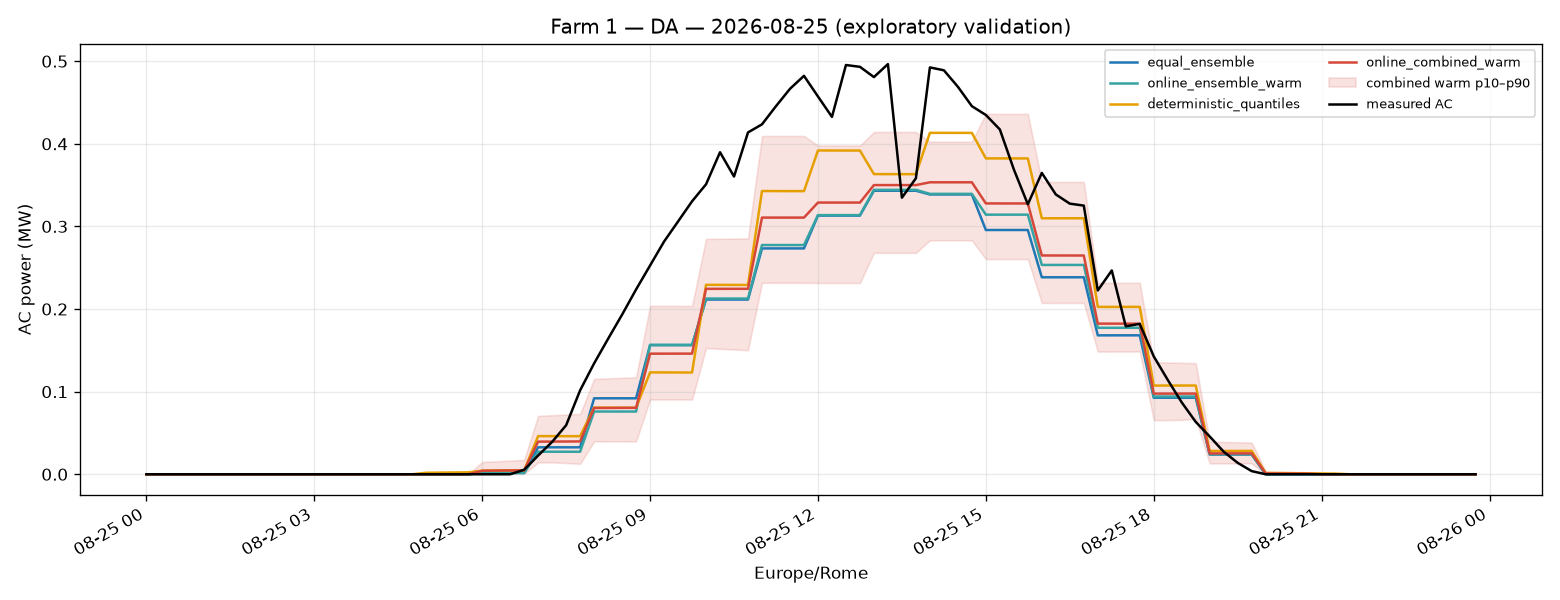
\includegraphics[width=0.97\textwidth]{docs/figures/pv_online_crps/farm_1_DA_forecast.png}\\[1em]
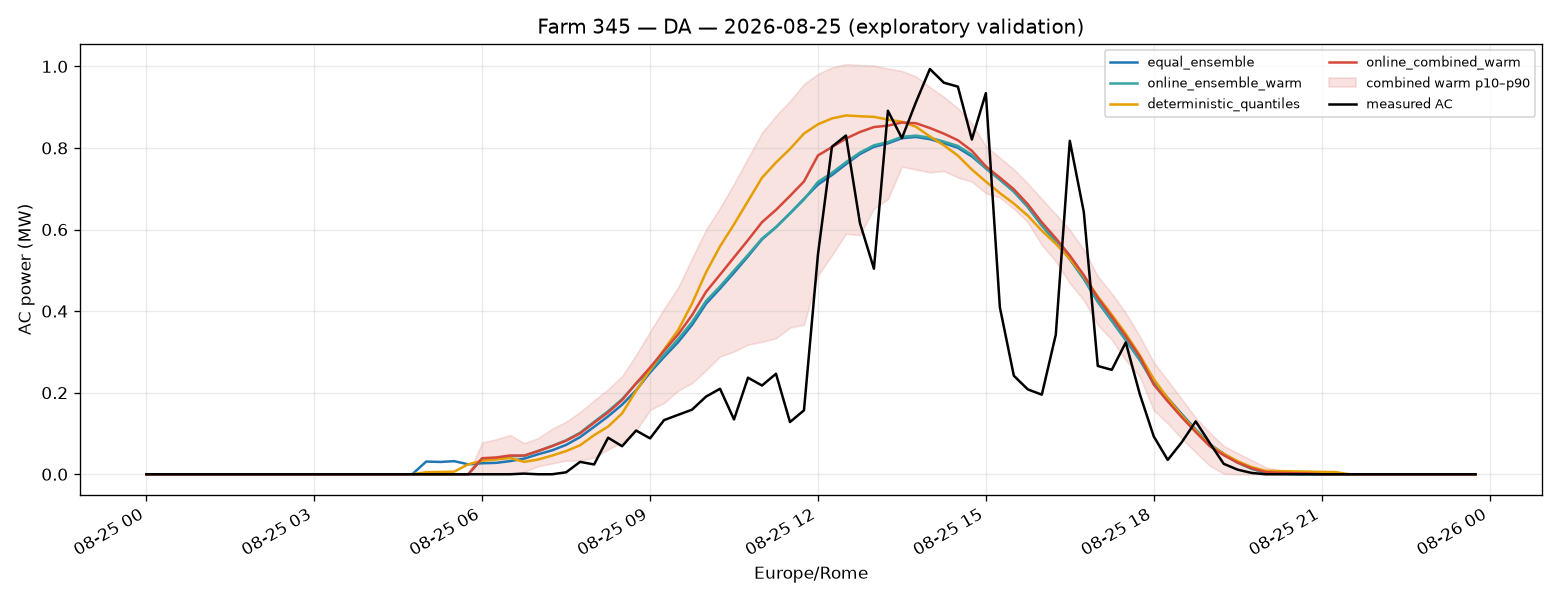
\includegraphics[width=0.97\textwidth]{docs/figures/pv_online_crps/farm_345_DA_forecast.png}
\caption{Illustrative DA forecast comparison on 25 August: farms 1 and 345.}\label{fig:forecast-a}\end{figure}
\begin{figure}[p]\centering
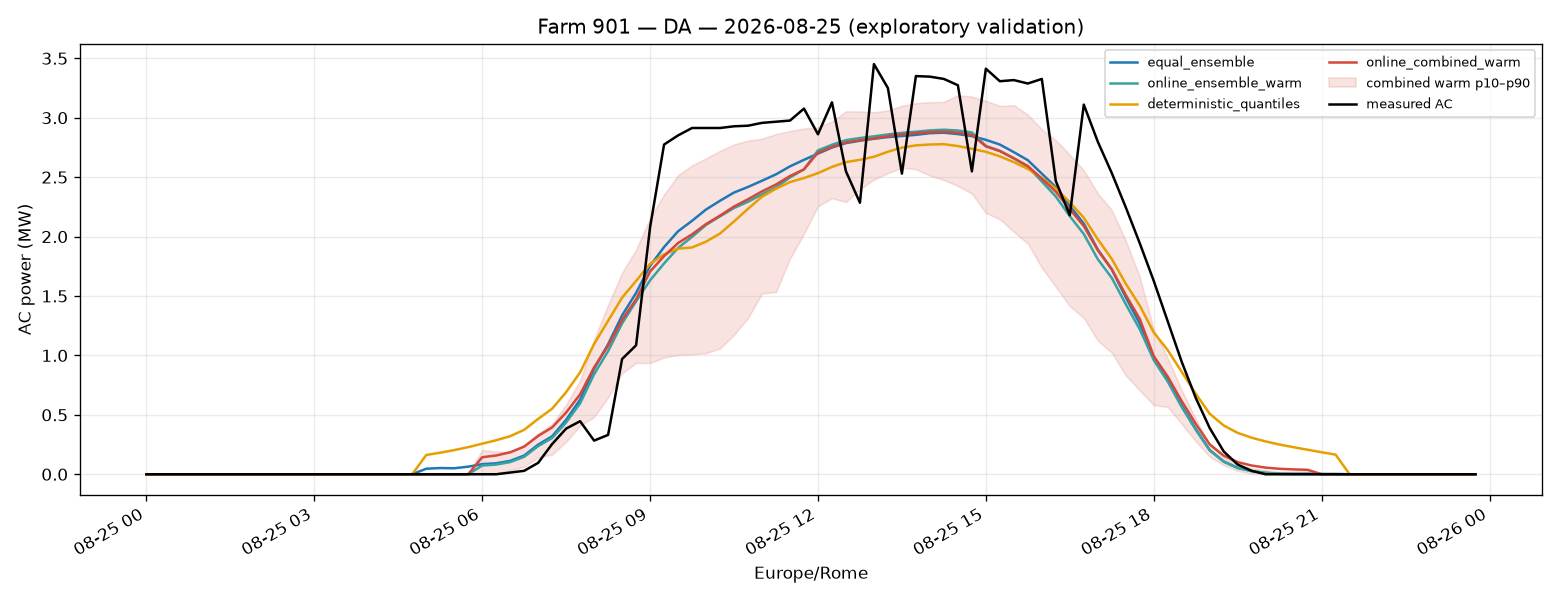
\includegraphics[width=0.97\textwidth]{docs/figures/pv_online_crps/farm_901_DA_forecast.png}\\[1em]
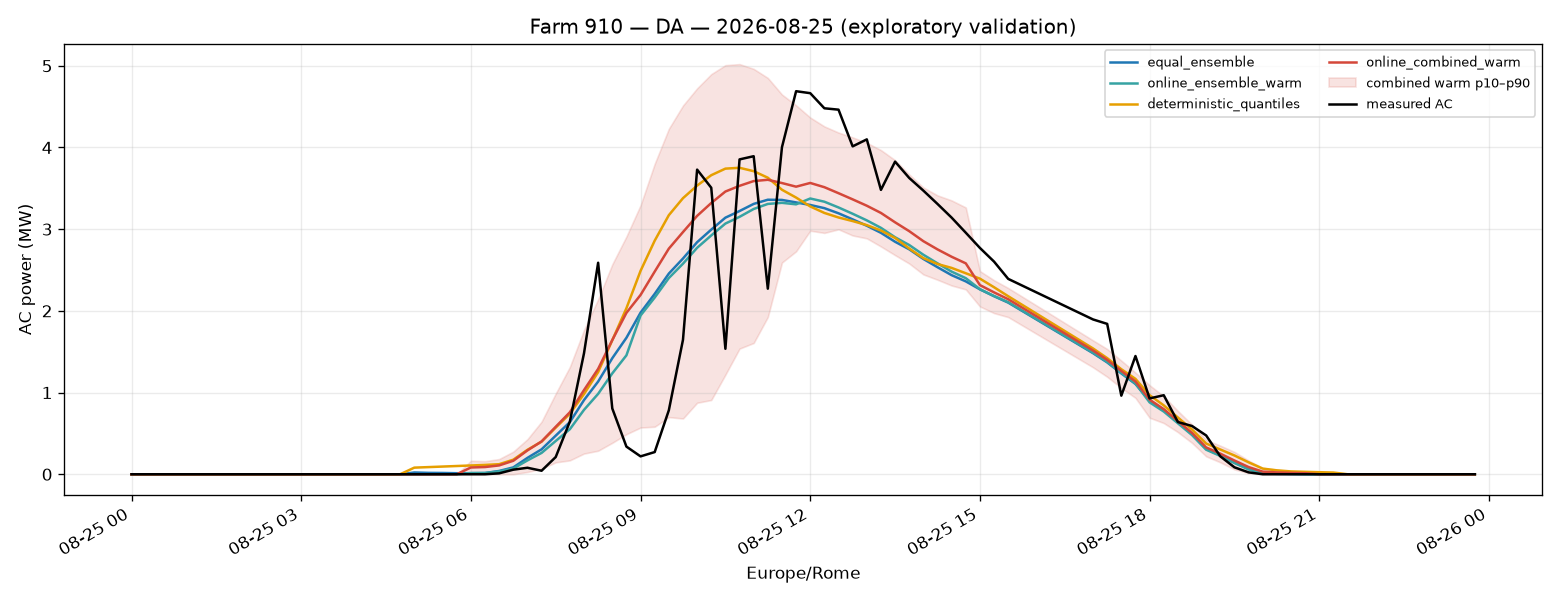
\includegraphics[width=0.97\textwidth]{docs/figures/pv_online_crps/farm_910_DA_forecast.png}
\caption{Illustrative DA forecast comparison on 25 August: farms 901 and 910.}\label{fig:forecast-b}\end{figure}
\clearpage
\subsection{Weight evolution}
Figures~\ref{fig:weights-a}--\ref{fig:weights-b} show the daily average DA pool weights and effective-expert counts. The deterministic \emph{point} line represents one expert, while the deterministic quantiles form a separate 19-expert group. Their weights should not be confused. For example, farm 1's warm DA deterministic point group changes from about 0.95\% to 0.65\% between the first and final validation days, while its deterministic-quantile group changes from approximately 46.5\% to 51.9\%. The grouping and uneven initialization make direct comparisons of source-group totals dependent on the number and correlation of experts.
\begin{figure}[p]\centering
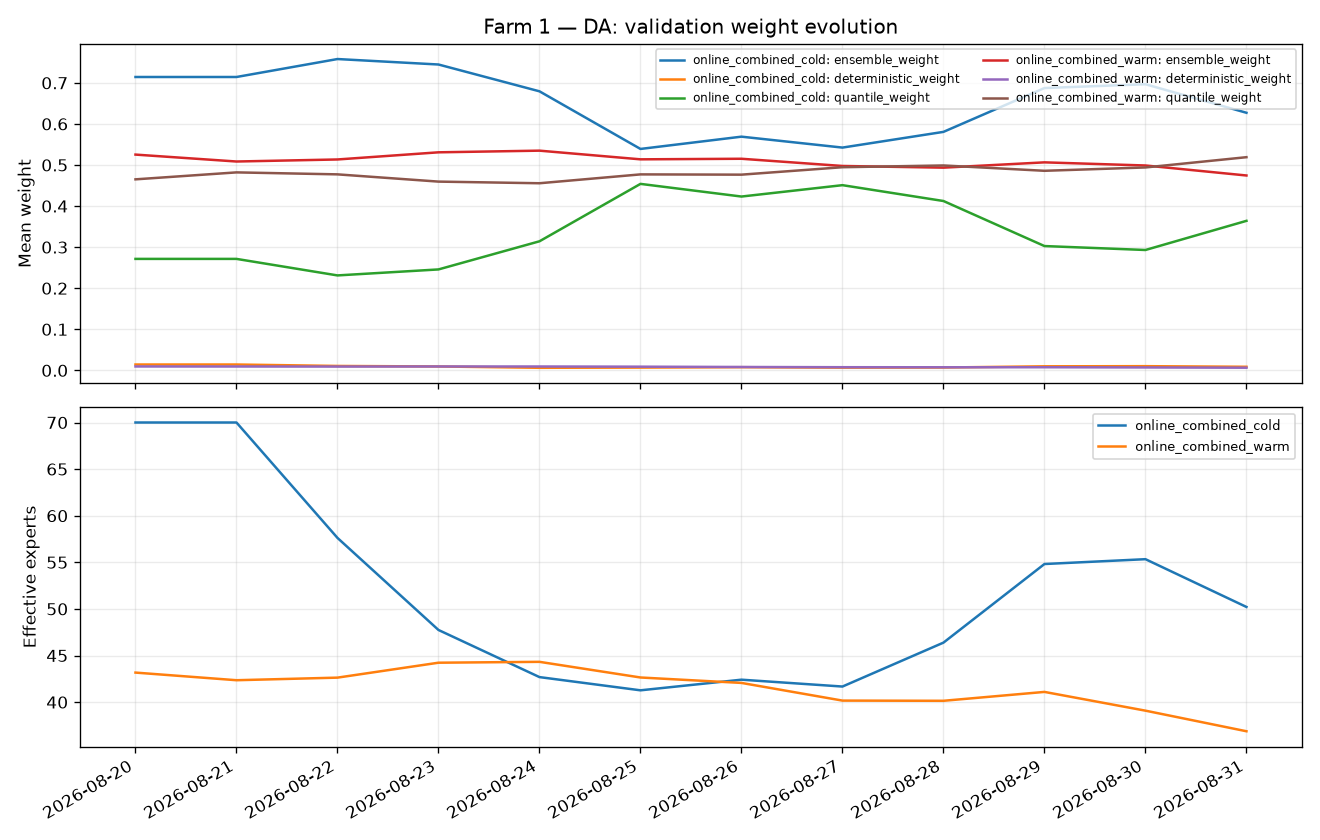
\includegraphics[width=0.93\textwidth]{docs/figures/pv_online_crps/farm_1_DA_weights.png}\\[1em]
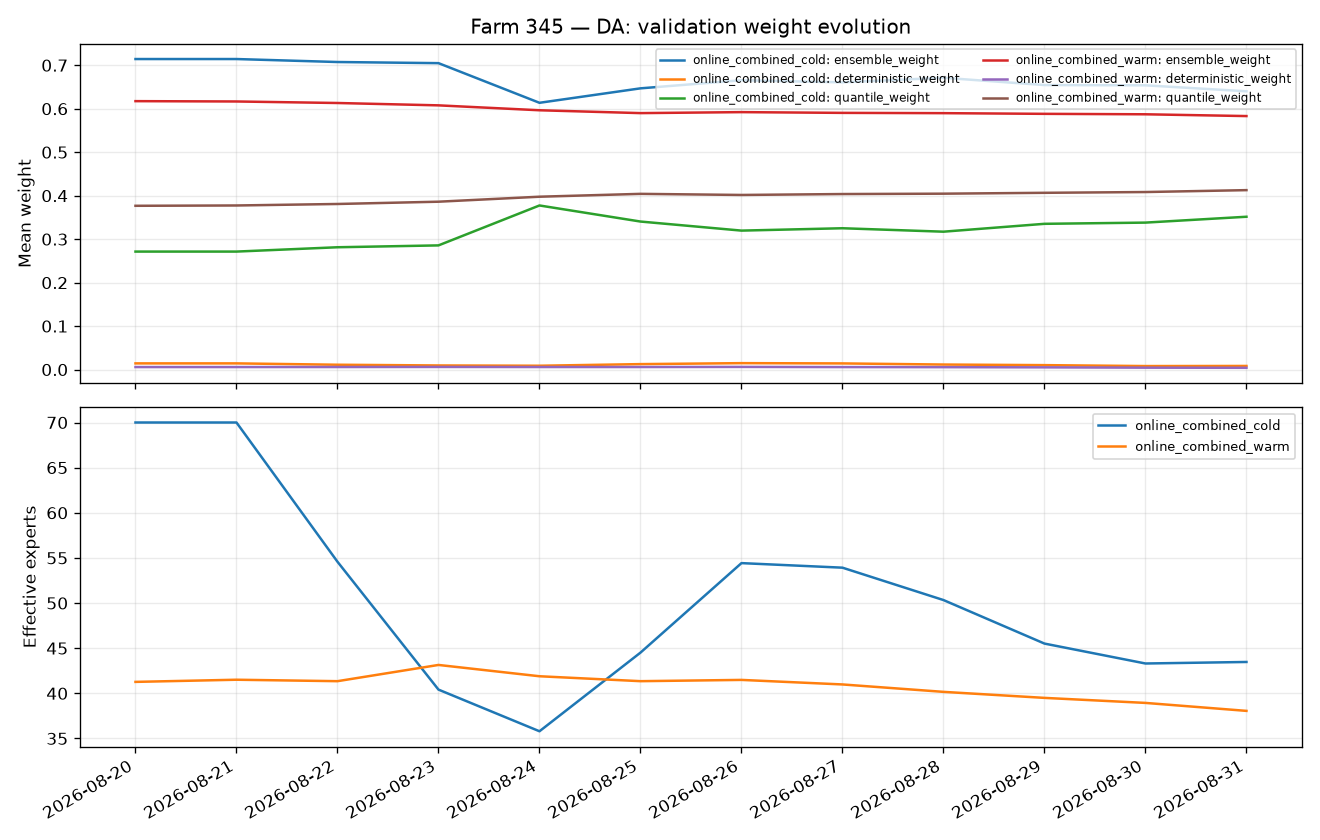
\includegraphics[width=0.93\textwidth]{docs/figures/pv_online_crps/farm_345_DA_weights.png}
\caption{DA combined-pool weight and effective-expert evolution: farms 1 and 345.}\label{fig:weights-a}\end{figure}
\begin{figure}[p]\centering
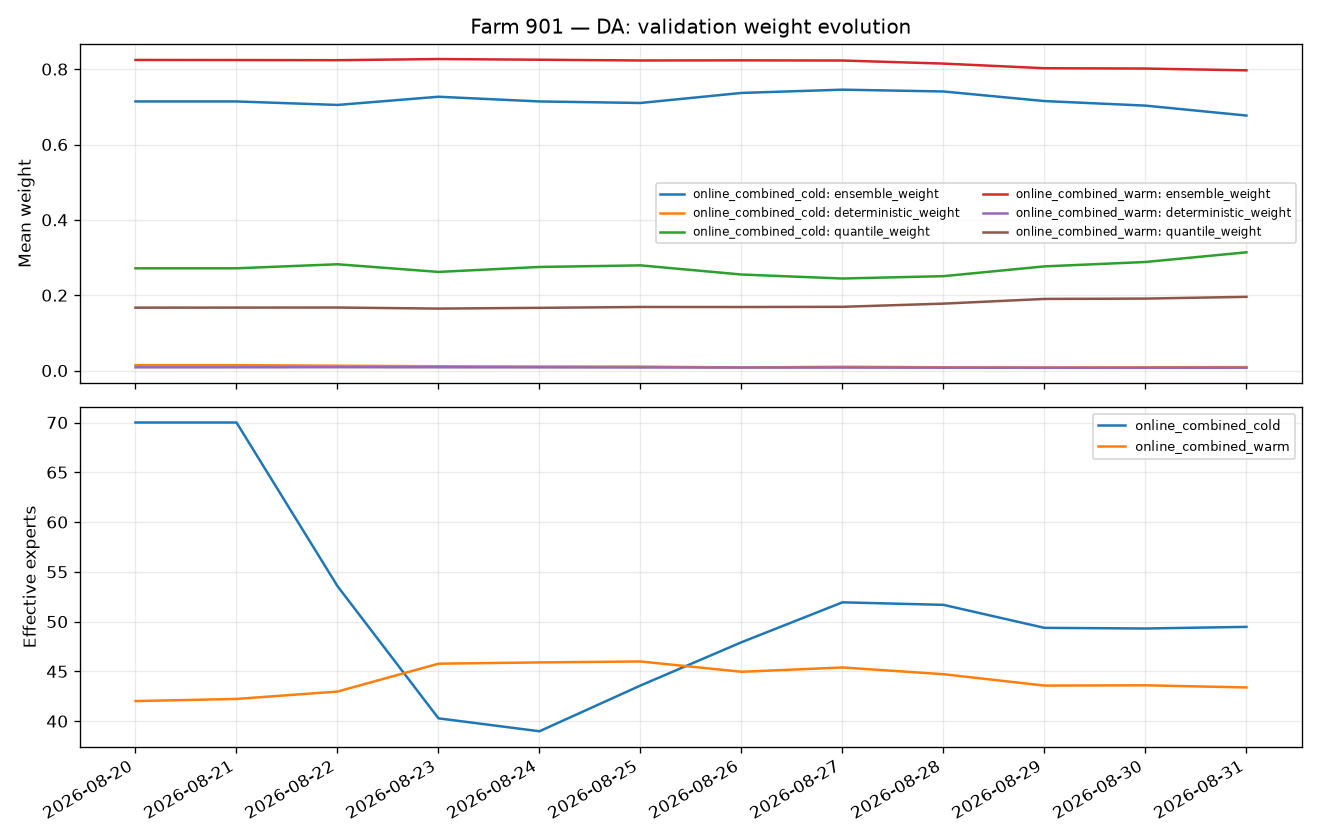
\includegraphics[width=0.93\textwidth]{docs/figures/pv_online_crps/farm_901_DA_weights.png}\\[1em]
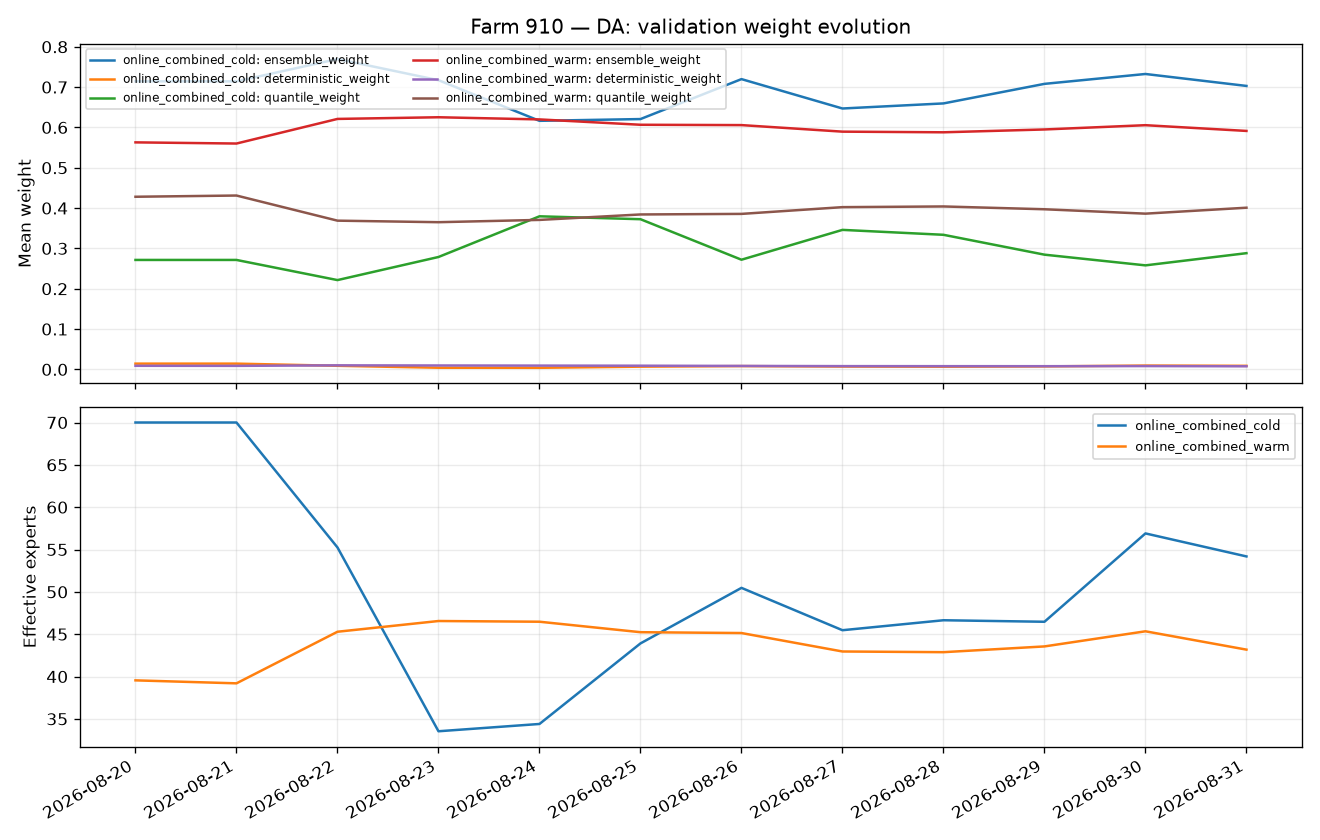
\includegraphics[width=0.93\textwidth]{docs/figures/pv_online_crps/farm_910_DA_weights.png}
\caption{DA combined-pool weight and effective-expert evolution: farms 901 and 910.}\label{fig:weights-b}\end{figure}
\clearpage
\section{Research limitations and future use}
\begin{enumerate}
\item \textbf{Model-selection bias and short validation:} candidates and online methods are examined on the same 12 days. Rankings and selected winners may be optimistic; 15-minute observations from the same day are dependent and do not represent independent daily weather events.
\item \textbf{Retrospective model availability:} the selected source models include August 19 targets and are not fully available at the first day's DA, IDA1 or IDA2 decision. No claim of a fully gate-causal backtest is made for those rows. All decisions also depend on the assumed six-hour weather and zero-minute target latency.
\item \textbf{Seasonality and sparse OOF history:} weather-model training contains January and August only. Deterministic error quantiles have seven-day minimum warm-up and may adapt using earlier validation outcomes. Extreme quantiles, block-specific weights and conclusions about seasonal transfer remain uncertain.
\item \textbf{Calibration and adjustments:} CRPS encourages accurate distributions but is not a guarantee that interval coverage is calibrated. Quantile crossings, physical clipping and the fixed night clock materially change predictions and are recorded. Target exclusions follow the approved file; the physical baseline uses 2025 fitted parameters as prior metadata.
\item \textbf{Dependent experts and initialization:} the 50 members share a model and weather ensemble; the 19 quantiles are derived from one deterministic forecast. Expert counts and correlations affect both initial source shares and effective-expert counts. The study does not identify causal importance of a forecast source.
\item \textbf{Trajectories and optimization:} independently ranked interval distributions and marginal quantiles do not specify temporal dependence or scenario paths, and the stochastic battery optimizer has not been supplied with a validated calibrated joint trajectory distribution by this study.
\item \textbf{Later datasets:} a future full-year 2026 ensemble archive should be inspected for issue cycles, six-hour availability assumptions, compatible member structure and matching curated measured power. Additional forecasts without measured targets do not create supervised evaluation examples. A separate chronological held-out period is needed before stronger operational claims.
\end{enumerate}

\section{Reproduction, outputs and checks}
The primary configurations are \code{configs/pv_experiments/probabilistic_january_august_2026.yaml} and \code{configs/pv_experiments/online_crps_january_august_2026.yaml}; both inherit \code{configs/standard.yaml}. \textbf{Do not launch or resume an experiment without first explaining the exact plan and obtaining the user's approval.} The following commands are for reference, subject to that approval:
\begin{lstlisting}
PYTHONPATH=src python scripts/study_pv_probabilistic.py \
  --config configs/pv_experiments/probabilistic_january_august_2026.yaml \
  --plan-only

PYTHONPATH=src python scripts/study_pv_online_crps.py \
  --config configs/pv_experiments/online_crps_january_august_2026.yaml \
  --plan-only

PYTHONPATH=src python scripts/study_pv_online_crps.py \
  --config configs/pv_experiments/online_crps_january_august_2026.yaml \
  --stage all --workers 42

PYTHONPATH=src python scripts/audit_pv_online_crps.py \
  --config configs/pv_experiments/online_crps_january_august_2026.yaml
\end{lstlisting}
The \code{prepare}, \code{evaluate}, and \code{report} stages can also be run separately. Preparation uses at most four farm processes and online evaluation at most sixteen farm/auction processes, below the requested cap of 42. The online outputs are rooted at \code{outputs/pv_online_crps/january_august_2026/}; they include prepared Parquet inputs, fold checkpoints, issued forecasts and weights, delayed-update logs, issue histories and correction counts, paired scored forecasts, metric and coverage tables, per-quantile reliability, spread--skill tables, weight summaries and daily plots. The committed compact results are under \code{docs/results/pv_online_crps_january_august_2026/}.

The existing \code{bess} environment inspected on 28 October 2026 contains Python 3.14.8, NumPy 2.5.4, pandas 3.0.6, scikit-learn 1.9.1, SciPy 1.18.1, xarray 2026.7.0, pvlib 0.16.1, PyTorch 2.14.1, LightGBM 4.7.0, CatBoost 1.2.10 and PyArrow 26.0.0. These are current inspection values, not a separately archived full runtime environment lockfile. No packages were installed for this document.

The focused software suite for this snapshot reported 71 passing tests across online CRPS, original probabilistic PV and configuration inheritance. The separate saved-artifact audit passed all 16 farm/auction combinations: deterministic forecasts respected their assumed availability, observation updates did not precede target availability, retrospective source forecasts did not train online weights, issued weights were probability vectors, deterministic quantiles were ordered and bounded, and IDA3 did not score pre-noon products. These checks validate the implemented contracts, not model accuracy or the assumptions themselves.

\begin{thebibliography}{9}
\bibitem{thorey2018} J. Thorey, C. Chaussin and V. Mallet, ``Ensemble forecast of photovoltaic power with online CRPS learning,'' \emph{International Journal of Forecasting}, vol. 34, pp. 762--773, 2018. DOI: \href{https://doi.org/10.1016/j.ijforecast.2018.05.007}{10.1016/j.ijforecast.2018.05.007}. User-provided copy: \code{docs/online_cprs_learning_forecasts.pdf}.
\end{thebibliography}
\end{document}
